\documentclass{article} % For LaTeX2e
\usepackage{iclr2027_conference,times}

% Optional math commands from https://github.com/goodfeli/dlbook_notation.
%%%%% NEW MATH DEFINITIONS %%%%%

\usepackage{amsmath,amsfonts,bm}

% Mark sections of captions for referring to divisions of figures
\newcommand{\figleft}{{\em (Left)}}
\newcommand{\figcenter}{{\em (Center)}}
\newcommand{\figright}{{\em (Right)}}
\newcommand{\figtop}{{\em (Top)}}
\newcommand{\figbottom}{{\em (Bottom)}}
\newcommand{\captiona}{{\em (a)}}
\newcommand{\captionb}{{\em (b)}}
\newcommand{\captionc}{{\em (c)}}
\newcommand{\captiond}{{\em (d)}}

% Highlight a newly defined term
\newcommand{\newterm}[1]{{\bf #1}}


% Figure reference, lower-case.
\def\figref#1{figure~\ref{#1}}
% Figure reference, capital. For start of sentence
\def\Figref#1{Figure~\ref{#1}}
\def\twofigref#1#2{figures \ref{#1} and \ref{#2}}
\def\quadfigref#1#2#3#4{figures \ref{#1}, \ref{#2}, \ref{#3} and \ref{#4}}
% Section reference, lower-case.
\def\secref#1{section~\ref{#1}}
% Section reference, capital.
\def\Secref#1{Section~\ref{#1}}
% Reference to two sections.
\def\twosecrefs#1#2{sections \ref{#1} and \ref{#2}}
% Reference to three sections.
\def\secrefs#1#2#3{sections \ref{#1}, \ref{#2} and \ref{#3}}
% Reference to an equation, lower-case.
\def\eqref#1{equation~\ref{#1}}
% Reference to an equation, upper case
\def\Eqref#1{Equation~\ref{#1}}
% A raw reference to an equation---avoid using if possible
\def\plaineqref#1{\ref{#1}}
% Reference to a chapter, lower-case.
\def\chapref#1{chapter~\ref{#1}}
% Reference to an equation, upper case.
\def\Chapref#1{Chapter~\ref{#1}}
% Reference to a range of chapters
\def\rangechapref#1#2{chapters\ref{#1}--\ref{#2}}
% Reference to an algorithm, lower-case.
\def\algref#1{algorithm~\ref{#1}}
% Reference to an algorithm, upper case.
\def\Algref#1{Algorithm~\ref{#1}}
\def\twoalgref#1#2{algorithms \ref{#1} and \ref{#2}}
\def\Twoalgref#1#2{Algorithms \ref{#1} and \ref{#2}}
% Reference to a part, lower case
\def\partref#1{part~\ref{#1}}
% Reference to a part, upper case
\def\Partref#1{Part~\ref{#1}}
\def\twopartref#1#2{parts \ref{#1} and \ref{#2}}

\def\ceil#1{\lceil #1 \rceil}
\def\floor#1{\lfloor #1 \rfloor}
\def\1{\bm{1}}
\newcommand{\train}{\mathcal{D}}
\newcommand{\valid}{\mathcal{D_{\mathrm{valid}}}}
\newcommand{\test}{\mathcal{D_{\mathrm{test}}}}

\def\eps{{\epsilon}}


% Random variables
\def\reta{{\textnormal{$\eta$}}}
\def\ra{{\textnormal{a}}}
\def\rb{{\textnormal{b}}}
\def\rc{{\textnormal{c}}}
\def\rd{{\textnormal{d}}}
\def\re{{\textnormal{e}}}
\def\rf{{\textnormal{f}}}
\def\rg{{\textnormal{g}}}
\def\rh{{\textnormal{h}}}
\def\ri{{\textnormal{i}}}
\def\rj{{\textnormal{j}}}
\def\rk{{\textnormal{k}}}
\def\rl{{\textnormal{l}}}
% rm is already a command, just don't name any random variables m
\def\rn{{\textnormal{n}}}
\def\ro{{\textnormal{o}}}
\def\rp{{\textnormal{p}}}
\def\rq{{\textnormal{q}}}
\def\rr{{\textnormal{r}}}
\def\rs{{\textnormal{s}}}
\def\rt{{\textnormal{t}}}
\def\ru{{\textnormal{u}}}
\def\rv{{\textnormal{v}}}
\def\rw{{\textnormal{w}}}
\def\rx{{\textnormal{x}}}
\def\ry{{\textnormal{y}}}
\def\rz{{\textnormal{z}}}

% Random vectors
\def\rvepsilon{{\mathbf{\epsilon}}}
\def\rvtheta{{\mathbf{\theta}}}
\def\rva{{\mathbf{a}}}
\def\rvb{{\mathbf{b}}}
\def\rvc{{\mathbf{c}}}
\def\rvd{{\mathbf{d}}}
\def\rve{{\mathbf{e}}}
\def\rvf{{\mathbf{f}}}
\def\rvg{{\mathbf{g}}}
\def\rvh{{\mathbf{h}}}
\def\rvu{{\mathbf{i}}}
\def\rvj{{\mathbf{j}}}
\def\rvk{{\mathbf{k}}}
\def\rvl{{\mathbf{l}}}
\def\rvm{{\mathbf{m}}}
\def\rvn{{\mathbf{n}}}
\def\rvo{{\mathbf{o}}}
\def\rvp{{\mathbf{p}}}
\def\rvq{{\mathbf{q}}}
\def\rvr{{\mathbf{r}}}
\def\rvs{{\mathbf{s}}}
\def\rvt{{\mathbf{t}}}
\def\rvu{{\mathbf{u}}}
\def\rvv{{\mathbf{v}}}
\def\rvw{{\mathbf{w}}}
\def\rvx{{\mathbf{x}}}
\def\rvy{{\mathbf{y}}}
\def\rvz{{\mathbf{z}}}

% Elements of random vectors
\def\erva{{\textnormal{a}}}
\def\ervb{{\textnormal{b}}}
\def\ervc{{\textnormal{c}}}
\def\ervd{{\textnormal{d}}}
\def\erve{{\textnormal{e}}}
\def\ervf{{\textnormal{f}}}
\def\ervg{{\textnormal{g}}}
\def\ervh{{\textnormal{h}}}
\def\ervi{{\textnormal{i}}}
\def\ervj{{\textnormal{j}}}
\def\ervk{{\textnormal{k}}}
\def\ervl{{\textnormal{l}}}
\def\ervm{{\textnormal{m}}}
\def\ervn{{\textnormal{n}}}
\def\ervo{{\textnormal{o}}}
\def\ervp{{\textnormal{p}}}
\def\ervq{{\textnormal{q}}}
\def\ervr{{\textnormal{r}}}
\def\ervs{{\textnormal{s}}}
\def\ervt{{\textnormal{t}}}
\def\ervu{{\textnormal{u}}}
\def\ervv{{\textnormal{v}}}
\def\ervw{{\textnormal{w}}}
\def\ervx{{\textnormal{x}}}
\def\ervy{{\textnormal{y}}}
\def\ervz{{\textnormal{z}}}

% Random matrices
\def\rmA{{\mathbf{A}}}
\def\rmB{{\mathbf{B}}}
\def\rmC{{\mathbf{C}}}
\def\rmD{{\mathbf{D}}}
\def\rmE{{\mathbf{E}}}
\def\rmF{{\mathbf{F}}}
\def\rmG{{\mathbf{G}}}
\def\rmH{{\mathbf{H}}}
\def\rmI{{\mathbf{I}}}
\def\rmJ{{\mathbf{J}}}
\def\rmK{{\mathbf{K}}}
\def\rmL{{\mathbf{L}}}
\def\rmM{{\mathbf{M}}}
\def\rmN{{\mathbf{N}}}
\def\rmO{{\mathbf{O}}}
\def\rmP{{\mathbf{P}}}
\def\rmQ{{\mathbf{Q}}}
\def\rmR{{\mathbf{R}}}
\def\rmS{{\mathbf{S}}}
\def\rmT{{\mathbf{T}}}
\def\rmU{{\mathbf{U}}}
\def\rmV{{\mathbf{V}}}
\def\rmW{{\mathbf{W}}}
\def\rmX{{\mathbf{X}}}
\def\rmY{{\mathbf{Y}}}
\def\rmZ{{\mathbf{Z}}}

% Elements of random matrices
\def\ermA{{\textnormal{A}}}
\def\ermB{{\textnormal{B}}}
\def\ermC{{\textnormal{C}}}
\def\ermD{{\textnormal{D}}}
\def\ermE{{\textnormal{E}}}
\def\ermF{{\textnormal{F}}}
\def\ermG{{\textnormal{G}}}
\def\ermH{{\textnormal{H}}}
\def\ermI{{\textnormal{I}}}
\def\ermJ{{\textnormal{J}}}
\def\ermK{{\textnormal{K}}}
\def\ermL{{\textnormal{L}}}
\def\ermM{{\textnormal{M}}}
\def\ermN{{\textnormal{N}}}
\def\ermO{{\textnormal{O}}}
\def\ermP{{\textnormal{P}}}
\def\ermQ{{\textnormal{Q}}}
\def\ermR{{\textnormal{R}}}
\def\ermS{{\textnormal{S}}}
\def\ermT{{\textnormal{T}}}
\def\ermU{{\textnormal{U}}}
\def\ermV{{\textnormal{V}}}
\def\ermW{{\textnormal{W}}}
\def\ermX{{\textnormal{X}}}
\def\ermY{{\textnormal{Y}}}
\def\ermZ{{\textnormal{Z}}}

% Vectors
\def\vzero{{\bm{0}}}
\def\vone{{\bm{1}}}
\def\vmu{{\bm{\mu}}}
\def\vtheta{{\bm{\theta}}}
\def\va{{\bm{a}}}
\def\vb{{\bm{b}}}
\def\vc{{\bm{c}}}
\def\vd{{\bm{d}}}
\def\ve{{\bm{e}}}
\def\vf{{\bm{f}}}
\def\vg{{\bm{g}}}
\def\vh{{\bm{h}}}
\def\vi{{\bm{i}}}
\def\vj{{\bm{j}}}
\def\vk{{\bm{k}}}
\def\vl{{\bm{l}}}
\def\vm{{\bm{m}}}
\def\vn{{\bm{n}}}
\def\vo{{\bm{o}}}
\def\vp{{\bm{p}}}
\def\vq{{\bm{q}}}
\def\vr{{\bm{r}}}
\def\vs{{\bm{s}}}
\def\vt{{\bm{t}}}
\def\vu{{\bm{u}}}
\def\vv{{\bm{v}}}
\def\vw{{\bm{w}}}
\def\vx{{\bm{x}}}
\def\vy{{\bm{y}}}
\def\vz{{\bm{z}}}

% Elements of vectors
\def\evalpha{{\alpha}}
\def\evbeta{{\beta}}
\def\evepsilon{{\epsilon}}
\def\evlambda{{\lambda}}
\def\evomega{{\omega}}
\def\evmu{{\mu}}
\def\evpsi{{\psi}}
\def\evsigma{{\sigma}}
\def\evtheta{{\theta}}
\def\eva{{a}}
\def\evb{{b}}
\def\evc{{c}}
\def\evd{{d}}
\def\eve{{e}}
\def\evf{{f}}
\def\evg{{g}}
\def\evh{{h}}
\def\evi{{i}}
\def\evj{{j}}
\def\evk{{k}}
\def\evl{{l}}
\def\evm{{m}}
\def\evn{{n}}
\def\evo{{o}}
\def\evp{{p}}
\def\evq{{q}}
\def\evr{{r}}
\def\evs{{s}}
\def\evt{{t}}
\def\evu{{u}}
\def\evv{{v}}
\def\evw{{w}}
\def\evx{{x}}
\def\evy{{y}}
\def\evz{{z}}

% Matrix
\def\mA{{\bm{A}}}
\def\mB{{\bm{B}}}
\def\mC{{\bm{C}}}
\def\mD{{\bm{D}}}
\def\mE{{\bm{E}}}
\def\mF{{\bm{F}}}
\def\mG{{\bm{G}}}
\def\mH{{\bm{H}}}
\def\mI{{\bm{I}}}
\def\mJ{{\bm{J}}}
\def\mK{{\bm{K}}}
\def\mL{{\bm{L}}}
\def\mM{{\bm{M}}}
\def\mN{{\bm{N}}}
\def\mO{{\bm{O}}}
\def\mP{{\bm{P}}}
\def\mQ{{\bm{Q}}}
\def\mR{{\bm{R}}}
\def\mS{{\bm{S}}}
\def\mT{{\bm{T}}}
\def\mU{{\bm{U}}}
\def\mV{{\bm{V}}}
\def\mW{{\bm{W}}}
\def\mX{{\bm{X}}}
\def\mY{{\bm{Y}}}
\def\mZ{{\bm{Z}}}
\def\mBeta{{\bm{\beta}}}
\def\mPhi{{\bm{\Phi}}}
\def\mLambda{{\bm{\Lambda}}}
\def\mSigma{{\bm{\Sigma}}}

% Tensor
\DeclareMathAlphabet{\mathsfit}{\encodingdefault}{\sfdefault}{m}{sl}
\SetMathAlphabet{\mathsfit}{bold}{\encodingdefault}{\sfdefault}{bx}{n}
\newcommand{\tens}[1]{\bm{\mathsfit{#1}}}
\def\tA{{\tens{A}}}
\def\tB{{\tens{B}}}
\def\tC{{\tens{C}}}
\def\tD{{\tens{D}}}
\def\tE{{\tens{E}}}
\def\tF{{\tens{F}}}
\def\tG{{\tens{G}}}
\def\tH{{\tens{H}}}
\def\tI{{\tens{I}}}
\def\tJ{{\tens{J}}}
\def\tK{{\tens{K}}}
\def\tL{{\tens{L}}}
\def\tM{{\tens{M}}}
\def\tN{{\tens{N}}}
\def\tO{{\tens{O}}}
\def\tP{{\tens{P}}}
\def\tQ{{\tens{Q}}}
\def\tR{{\tens{R}}}
\def\tS{{\tens{S}}}
\def\tT{{\tens{T}}}
\def\tU{{\tens{U}}}
\def\tV{{\tens{V}}}
\def\tW{{\tens{W}}}
\def\tX{{\tens{X}}}
\def\tY{{\tens{Y}}}
\def\tZ{{\tens{Z}}}


% Graph
\def\gA{{\mathcal{A}}}
\def\gB{{\mathcal{B}}}
\def\gC{{\mathcal{C}}}
\def\gD{{\mathcal{D}}}
\def\gE{{\mathcal{E}}}
\def\gF{{\mathcal{F}}}
\def\gG{{\mathcal{G}}}
\def\gH{{\mathcal{H}}}
\def\gI{{\mathcal{I}}}
\def\gJ{{\mathcal{J}}}
\def\gK{{\mathcal{K}}}
\def\gL{{\mathcal{L}}}
\def\gM{{\mathcal{M}}}
\def\gN{{\mathcal{N}}}
\def\gO{{\mathbf{0}}}
\def\gP{{\mathcal{P}}}
\def\gQ{{\mathcal{Q}}}
\def\gR{{\mathcal{R}}}
\def\gS{{\mathcal{S}}}
\def\gT{{\mathcal{T}}}
\def\gU{{\mathcal{U}}}
\def\gV{{\mathcal{V}}}
\def\gW{{\mathcal{W}}}
\def\gX{{\mathcal{X}}}
\def\gY{{\mathcal{Y}}}
\def\gZ{{\mathcal{Z}}}

% Sets
\def\sA{{\mathbb{A}}}
\def\sB{{\mathbb{B}}}
\def\sC{{\mathbb{C}}}
\def\sD{{\mathbb{D}}}
% Don't use a set called E, because this would be the same as our symbol
% for expectation.
\def\sF{{\mathbb{F}}}
\def\sG{{\mathbb{G}}}
\def\sH{{\mathbb{H}}}
\def\sI{{\mathbb{I}}}
\def\sJ{{\mathbb{J}}}
\def\sK{{\mathbb{K}}}
\def\sL{{\mathbb{L}}}
\def\sM{{\mathbb{M}}}
\def\sN{{\mathbb{N}}}
\def\sO{{\mathbb{O}}}
\def\sP{{\mathbb{P}}}
\def\sQ{{\mathbb{Q}}}
\def\sR{{\mathbb{R}}}
\def\sS{{\mathbb{S}}}
\def\sT{{\mathbb{T}}}
\def\sU{{\mathbb{U}}}
\def\sV{{\mathbb{V}}}
\def\sW{{\mathbb{W}}}
\def\sX{{\mathbb{X}}}
\def\sY{{\mathbb{Y}}}
\def\sZ{{\mathbb{Z}}}

% Entries of a matrix
\def\emLambda{{\Lambda}}
\def\emA{{A}}
\def\emB{{B}}
\def\emC{{C}}
\def\emD{{D}}
\def\emE{{E}}
\def\emF{{F}}
\def\emG{{G}}
\def\emH{{H}}
\def\emI{{I}}
\def\emJ{{J}}
\def\emK{{K}}
\def\emL{{L}}
\def\emM{{M}}
\def\emN{{N}}
\def\emO{{O}}
\def\emP{{P}}
\def\emQ{{Q}}
\def\emR{{R}}
\def\emS{{S}}
\def\emT{{T}}
\def\emU{{U}}
\def\emV{{V}}
\def\emW{{W}}
\def\emX{{X}}
\def\emY{{Y}}
\def\emZ{{Z}}
\def\emSigma{{\Sigma}}

% entries of a tensor
% Same font as tensor, without \bm wrapper
\newcommand{\etens}[1]{\mathsfit{#1}}
\def\etLambda{{\etens{\Lambda}}}
\def\etA{{\etens{A}}}
\def\etB{{\etens{B}}}
\def\etC{{\etens{C}}}
\def\etD{{\etens{D}}}
\def\etE{{\etens{E}}}
\def\etF{{\etens{F}}}
\def\etG{{\etens{G}}}
\def\etH{{\etens{H}}}
\def\etI{{\etens{I}}}
\def\etJ{{\etens{J}}}
\def\etK{{\etens{K}}}
\def\etL{{\etens{L}}}
\def\etM{{\etens{M}}}
\def\etN{{\etens{N}}}
\def\etO{{\etens{O}}}
\def\etP{{\etens{P}}}
\def\etQ{{\etens{Q}}}
\def\etR{{\etens{R}}}
\def\etS{{\etens{S}}}
\def\etT{{\etens{T}}}
\def\etU{{\etens{U}}}
\def\etV{{\etens{V}}}
\def\etW{{\etens{W}}}
\def\etX{{\etens{X}}}
\def\etY{{\etens{Y}}}
\def\etZ{{\etens{Z}}}

% The true underlying data generating distribution
\newcommand{\pdata}{p_{\rm{data}}}
% The empirical distribution defined by the training set
\newcommand{\ptrain}{\hat{p}_{\rm{data}}}
\newcommand{\Ptrain}{\hat{P}_{\rm{data}}}
% The model distribution
\newcommand{\pmodel}{p_{\rm{model}}}
\newcommand{\Pmodel}{P_{\rm{model}}}
\newcommand{\ptildemodel}{\tilde{p}_{\rm{model}}}
% Stochastic autoencoder distributions
\newcommand{\pencode}{p_{\rm{encoder}}}
\newcommand{\pdecode}{p_{\rm{decoder}}}
\newcommand{\precons}{p_{\rm{reconstruct}}}

\newcommand{\laplace}{\mathrm{Laplace}} % Laplace distribution

\newcommand{\E}{\mathbb{E}}
\newcommand{\Ls}{\mathcal{L}}
\newcommand{\R}{\mathbb{R}}
\newcommand{\emp}{\tilde{p}}
\newcommand{\lr}{\alpha}
\newcommand{\reg}{\lambda}
\newcommand{\rect}{\mathrm{rectifier}}
\newcommand{\softmax}{\mathrm{softmax}}
\newcommand{\sigmoid}{\sigma}
\newcommand{\softplus}{\zeta}
\newcommand{\KL}{D_{\mathrm{KL}}}
\newcommand{\Var}{\mathrm{Var}}
\newcommand{\standarderror}{\mathrm{SE}}
\newcommand{\Cov}{\mathrm{Cov}}
% Wolfram Mathworld says $L^2$ is for function spaces and $\ell^2$ is for vectors
% But then they seem to use $L^2$ for vectors throughout the site, and so does
% wikipedia.
\newcommand{\normlzero}{L^0}
\newcommand{\normlone}{L^1}
\newcommand{\normltwo}{L^2}
\newcommand{\normlp}{L^p}
\newcommand{\normmax}{L^\infty}

\newcommand{\parents}{Pa} % See usage in notation.tex. Chosen to match Daphne's book.

\DeclareMathOperator*{\argmax}{arg\,max}
\DeclareMathOperator*{\argmin}{arg\,min}

\DeclareMathOperator{\sign}{sign}
\DeclareMathOperator{\Tr}{Tr}
\let\ab\allowbreak


\usepackage{hyperref}
\usepackage{url}
\usepackage{graphicx}
\usepackage{capt-of}
\usepackage{array}
\usepackage{booktabs}
\usepackage{amssymb}
\usepackage[table]{xcolor}
\usepackage{arydshln}
\usepackage{wrapfig}
\usepackage{needspace}
\usepackage{fvextra}
\usepackage[breakable,skins]{tcolorbox}
\usepackage{ragged2e}
\usetikzlibrary{positioning,arrows.meta}
\definecolor{experiencepurple}{HTML}{F5F2FA}
\definecolor{experienceyellow}{HTML}{FFFAEE}
\definecolor{dialogueblue}{HTML}{F1F7FA}
\definecolor{changeaccent}{HTML}{B22222}
\tcbset{experience/.style={enhanced,breakable,boxrule=0.4pt,arc=2pt,
  colframe=black!25,colbacktitle=white,coltitle=black,fonttitle=\bfseries\small,
  left=7pt,right=7pt,top=3pt,bottom=3pt,before skip=8pt,after skip=8pt}}
\newtcolorbox{MessageBox}[3][]{experience,unbreakable,colback=#2,title={#3},fonttitle=\sffamily\bfseries\TraceFont,fontupper=\sffamily\TraceFont,boxsep=1pt,left=4pt,right=4pt,top=1pt,bottom=1pt,toptitle=1pt,bottomtitle=1pt,before skip=2pt,after skip=2pt,before upper={\setlength{\parskip}{0pt}},width=\linewidth,#1}
\tcbset{agent message/.style={width=0.97\linewidth,flush left,top=0pt,bottom=0pt,before skip=1pt,after skip=1pt},
  other message/.style={width=0.97\linewidth,flush right,top=0pt,bottom=0pt,before skip=1pt,after skip=1pt},
  loaded skill/.style={colframe=violet!50!black,colbacktitle=violet!12,boxrule=0.7pt}}
\newtcolorbox{ExecutionBox}[4][]{enhanced,unbreakable,colback=white,colframe=#2,colbacktitle=#3,coltitle=black,title={#4},fonttitle=\bfseries\small,boxrule=0.8pt,arc=2pt,boxsep=1pt,left=3pt,right=3pt,top=1pt,bottom=1pt,toptitle=1pt,bottomtitle=1pt,before skip=3pt,after skip=3pt,before upper={\setlength{\parskip}{0pt}},#1}
\newcommand{\TraceFont}{\fontsize{8}{9.5}\selectfont}
\DefineVerbatimEnvironment{Trajectory}{Verbatim}{fontsize=\TraceFont,fontfamily=phv,formatcom={\fontencoding{T1}\selectfont},breaklines=true,breakanywhere=false,breaksymbolleft={},breaksymbolright={},breakindent=0pt,breakautoindent=false,listparameters={\setlength{\topsep}{0pt}\setlength{\partopsep}{0pt}}}
\newtcolorbox{VideoStrip}{enhanced,colback=black!8,frame hidden,sharp corners,boxrule=0pt,
  boxsep=0pt,left=0pt,right=0pt,top=0pt,bottom=0pt,before skip=0pt,after skip=2pt}
\newcommand{\VideoStripFrame}[1]{\includegraphics[width=\dimexpr(\linewidth-6pt)/4\relax]{#1}}
\newcommand{\VideoStripLabel}[1]{\parbox[t]{\dimexpr(\linewidth-6pt)/4\relax}{\centering\sffamily\fontsize{7}{8}\selectfont\color{black!65}#1}}
% Table definitions. Load once with % Table definitions. Load once with % Table definitions. Load once with \input{table} in the preamble.
% Invoke individual table commands in the experiments or supplementary material.
% Optional argument: rendered table width, e.g. \VideoSpyMedicalTable[0.9\linewidth].
% Defaults preserve current widths; \width keeps the natural table width.
% Requires array, booktabs, amssymb, graphicx, arydshln, wrapfig, and xcolor with the table option.
\definecolor{videospyblue}{RGB}{235,245,252}
\definecolor{videospygreen}{RGB}{244,250,244}

% Equal padding above and below every dashed separator.
\newcommand{\VideoSpyDashLine}{%
\noalign{\vskip 1pt}\hdashline\noalign{\vskip 1pt}}

\newcommand{\VideoSpySetupTable}[1][0.9\linewidth]{%
\begin{table}[!t]
\centering
\caption{Datasets, evaluation splits, and metrics. MCQ: multiple-choice questions.}
\label{tab:data_splits}
\vspace{4pt}
\small
\setlength{\tabcolsep}{3pt}
\renewcommand{\arraystretch}{1.05}
\resizebox{#1}{!}{%
\begin{tabular}{@{}>{\raggedright\arraybackslash}p{.19\linewidth}
>{\raggedright\arraybackslash}p{.18\linewidth}
>{\raggedright\arraybackslash}p{.16\linewidth}
>{\raggedright\arraybackslash}p{.24\linewidth}
>{\raggedright\arraybackslash}p{.16\linewidth}@{}}
\toprule
Benchmark & Tasks & Training & Test & Main metrics \\
\midrule
LVBench\newline\citep{wang2025lvbench} & Long-video MCQ (6 types) & 83 videos /\newline 1,234 questions & 20 videos /\newline 315 questions & Overall, per-type accuracy \\
\addlinespace[2pt]
EgoLifeQA\newline\citep{yang2025egolife} & Egocentric video MCQ (5 types) & Days 1--5 /\newline 405 questions & Days 6--7 /\newline 95 questions & Overall, per-type accuracy \\
\addlinespace[2pt]
MedVidBench\newline\citep{su2026medgrpo} & Medical video tasks (8 types) & 5,146 tasks & Local: 1,124 tasks\newline Leaderboard: 6,245 tasks & 10 official task metrics \\
\bottomrule
\end{tabular}%
}
\end{table}
%
}

\newcommand{\VideoSpyAblationTable}[1][0.86\linewidth]{%
\begin{table}[!t]
\centering
\caption{Ablations of the evolution framework with Qwen3.5-4B. Checkmarks indicate enabled components. Bold marks the best result in each metric column.}
\label{tab:ablation}
\vspace{4pt}
\small
\setlength{\tabcolsep}{1.5pt}
\renewcommand{\arraystretch}{1.05}
\resizebox{#1}{!}{%
\begin{tabular}{@{}lccccrrrrrr@{}}
\toprule
Configuration & \multicolumn{2}{c}{Reflector} & \multicolumn{2}{c}{Agent Optimizer} & \multicolumn{3}{c}{LVBench} & \multicolumn{3}{c}{EgoLifeQA} \\
\cmidrule(lr){2-3}\cmidrule(lr){4-5}\cmidrule(lr){6-8}\cmidrule(l){9-11}
 & \shortstack{Task-grouped\\reflection} & \shortstack{Evidence-based\\review} & Skill & Memory & \shortstack{Acc. \\(\%)} $\uparrow$ & \shortstack{Avg. \\rounds $\downarrow$}  & \shortstack{Avg. \\tokens $\downarrow$} & \shortstack{Acc. \\(\%)} $\uparrow$ & \shortstack{Avg. \\rounds $\downarrow$}  & \shortstack{Avg. \\tokens $\downarrow$} \\
\midrule
\rowcolor{videospyblue}
VideoSpy$^{\mathbf{0}}$ & -- & -- & -- & -- & 39.4 & 11.7 & 80.3k & 32.6 & 14.7 & 129.0k \\
\midrule
\multicolumn{11}{@{}l}{\colorbox{videospygreen}{\textit{(a) Reflector}}} \\
Skill only (ungrouped) & -- & $\checkmark$ & $\checkmark$ & -- & 36.5 & 12.4 & 83.2k & 31.6 & 14.9 & 135.5k \\
Skill+Memory (no review) & $\checkmark$ & -- & $\checkmark$ & $\checkmark$ & 39.7 & 12.8 & 84.5k & 33.7 & 15.2 & 139.3k \\
\midrule
\multicolumn{11}{@{}l}{\colorbox{videospygreen}{\textit{(b) Agent Optimizer}}} \\
Skill only & $\checkmark$ & $\checkmark$ & $\checkmark$ & -- & 41.3 & 9.8 & 74.2k & 34.7 & 12.2 & 121.5k \\
Memory only & $\checkmark$ & $\checkmark$ & -- & $\checkmark$ & 40.3 & 10.9 & 77.7k & 34.7 & 13.1 & 129.8k \\
\rowcolor{videospyblue}
VideoSpy$^{\mathcal{E}}$ & $\checkmark$ & $\checkmark$ & $\checkmark$ & $\checkmark$ & \textbf{43.2} & \textbf{9.3} & \textbf{69.7k} & \textbf{36.8} & \textbf{11.7} & \textbf{116.5k} \\
\bottomrule
\end{tabular}%
}
\end{table}
%
}


\newcommand{\VideoSpyVisualToolsTable}[1][\linewidth]{%
\begin{table}[ht]
\centering
\caption{Visual-tool configurations of the foundational agent with Qwen3.5-4B, before evolution. Checkmarks indicate available tools; -- indicates a disabled tool. All configurations have no loaded Skill or Memory. Bold marks the best value in each metric column.}
\label{tab:visual_tools}
\vspace{4pt}
\small
\setlength{\tabcolsep}{2pt}
\renewcommand{\arraystretch}{1.1}
\resizebox{#1}{!}{%
\begin{tabular}{@{}lcccrrrrrr@{}}
\toprule
Configuration & \multicolumn{3}{c}{Available visual tools} & \multicolumn{3}{c}{LVBench} & \multicolumn{3}{c}{EgoLifeQA} \\
\cmidrule(lr){2-4}\cmidrule(lr){5-7}\cmidrule(l){8-10}
 & \texttt{overview} & \texttt{clip\_skim} & \texttt{frame\_inspect} & \shortstack{Acc. \\(\%)} $\uparrow$ & \shortstack{Avg. \\rounds $\downarrow$} & \shortstack{Avg. \\tokens $\downarrow$} & \shortstack{Acc. \\(\%)} $\uparrow$ & \shortstack{Avg. \\rounds $\downarrow$} & \shortstack{Avg. \\tokens $\downarrow$} \\
 \midrule
\texttt{overview} only & $\checkmark$ & -- & -- & 33.7 & \textbf{6.1} & \textbf{44.6k} & 26.3 & \textbf{8.5} & \textbf{100.4k} \\
Without \texttt{frame\_inspect} & $\checkmark$ & $\checkmark$ & -- & 36.8 & 9.5 & 62.9k & 30.5 & 12.3 & 115.2k \\
Without \texttt{clip\_skim} & $\checkmark$ & -- & $\checkmark$ & 37.5 & 10.8 & 69.7k & 29.5 & 13.7 & 134.8k \\
\midrule
VideoSpy$^{\mathbf{0}}$ (full tools) & $\checkmark$ & $\checkmark$ & $\checkmark$ & \textbf{39.4} & 11.7 & 80.3k & \textbf{32.6} & 14.7 & 129.0k \\
\bottomrule
\end{tabular}%
}
\end{table}%
}


\newcommand{\VideoSpyComparisonTable}[1][0.86\linewidth]{%
\begin{table}[!t]
\centering
\caption{Accuracy and inference cost on LVBench and EgoLifeQA. Bold marks the best value in each metric column within the online group (b). $^*$ denotes reproduced baselines (Avg. tokens cost per task for prebuilt indices (LVBench/EgoLifeQA): DVDAgent 14.1k/23.9k (reused GPT-4.1-generated LVBench captions), WorldMM 405.7k/reused).}
\label{tab:method_comparison}
\vspace{4pt}
\small
\setlength{\tabcolsep}{4pt}
\renewcommand{\arraystretch}{1.05}
\resizebox{#1}{!}{%
\begin{tabular}{llrrrrrr}
\toprule
Method & Model & \multicolumn{3}{c}{LVBench} & \multicolumn{3}{c}{EgoLifeQA} \\
\cmidrule(lr){3-5}\cmidrule(l){6-8}
 &  & Acc. (\%) $\uparrow$ & Avg. rounds $\downarrow$ & Avg. tokens $\downarrow$ & Acc. (\%) $\uparrow$ & Avg. rounds $\downarrow$ & Avg. tokens $\downarrow$ \\
\midrule
\multicolumn{8}{@{}l}{\colorbox{videospygreen}{\textit{(a) Offline caption or memory construction (requires a prebuilt text index)}}} \\
DVDAgent\textsuperscript{*}~{\scriptsize\citep{zhang2025dvd}} & 4B & 55.9 & 10.6 & 437.5k & 33.7 & 14.1 & 104.3k \\
WorldMM\textsuperscript{*}~{\scriptsize\citep{yeo2026worldmm}} & 4B & 36.5 & 2.9 & 39.1k & 37.9 & 2.7 & 25.8k \\
\midrule
\multicolumn{8}{@{}l}{\colorbox{videospygreen}{\textit{(b) Online active evidence gathering (raw video, no offline index)}}} \\
VideoSeek\textsuperscript{*}~{\scriptsize\citep{lin2026videoseek}} & 4B & 33.7 & 10.9 & 244.9k & 26.3 & 13.3 & 202.5k \\
% \VideoSpyDashLine
\rowcolor{videospyblue}
VideoSpy$^{\mathbf{0}}$ {\scriptsize\textit{(ours)}} & 4B & 39.4 & 11.7 & 80.3k & 32.6 & 14.7 & 129.0k \\
\rowcolor{videospyblue}
VideoSpy$^{\mathcal{E}}$ {\scriptsize\textit{(ours)}} & 4B & 43.2 & \textbf{9.3} & \textbf{69.7k} & 36.8 & 11.7 & 116.5k \\
\rowcolor{videospyblue}
VideoSpy$^{\mathbf{0}}$ {\scriptsize\textit{(ours)}} & 27B & 56.8 & 11.0 & 86.2k & 41.1 & 12.1 & 102.5k \\
\rowcolor{videospyblue}
VideoSpy$^{\mathcal{E}}$ {\scriptsize\textit{(ours)}} & 27B & \textbf{60.6} & 10.2 & 71.1k & \textbf{42.1} & \textbf{11.2} & \textbf{100.2k} \\
\bottomrule
\end{tabular}%
}
\end{table}
%
}

\newcommand{\VideoSpyMedicalTable}[1][\linewidth]{%
\begin{table}[!t]
\centering
\caption{MedVidBench results on local and leaderboard splits. All leaderboard baselines use 1-shot prompting. Bold marks the best value in each metric column within each split. $^*$ denotes reproduced baselines (Avg. tokens cost per task for prebuilt indices: DVDAgent 183.2k, WorldMM 174.5k.)}
\label{tab:medical_comparison}
\vspace{4pt}
\scriptsize
\setlength{\tabcolsep}{2.5pt}
\renewcommand{\arraystretch}{1.1}
\resizebox{#1}{!}{%
\begin{tabular}{llrrrrrrrrrr}
\toprule
Method & Model & CVS acc & NAP acc & SA acc & STG mIoU & TAG$_{\mathrm{mIoU}}$@0.3 & TAG$_{\mathrm{mIoU}}$@0.5 & DVC F1 & DVC llm & VS llm & RC llm \\
\midrule
\multicolumn{12}{@{}l}{\colorbox{videospygreen}{\textit{(a) Local test split (1,124 samples).}}} \\
DVDAgent\textsuperscript{*}~{\tiny\citep{zhang2025dvd}} & 4B & 0.205 & 0.169 & 0.080 & 0.031 & 0.027 & 0.024 & 0.121 & 2.184 & 3.925 & 2.708 \\
WorldMM\textsuperscript{*}~{\tiny\citep{yeo2026worldmm}} & 4B & 0.732 & 0.202 & 0.204 & 0.011 & 0.028 & 0.012 & 0.156 & 1.790 & 2.760 & 1.640 \\
VideoSeek\textsuperscript{*}~{\tiny\citep{lin2026videoseek}} & 4B & 0.289 & 0.274 & \textbf{0.225} & 0.033 & 0.185 & 0.157 & 0.184 & 2.061 & 1.754 & 2.204 \\
% \VideoSpyDashLine
\rowcolor{videospyblue}
VideoSpy$^{\mathbf{0}}$ {\tiny\textit{(ours)}} & 4B & 0.393 & 0.250 & 0.000 & 0.049 & 0.232 & 0.177 & 0.227 & 1.835 & 3.036 & 3.044 \\
\rowcolor{videospyblue}
VideoSpy$^{\mathcal{E}}$ {\tiny\textit{(ours)}} & 4B & 0.581 & \textbf{0.325} & 0.000 & 0.036 & 0.212 & 0.166 & 0.232 & 1.972 & 3.224 & 3.422 \\
\rowcolor{videospyblue}
VideoSpy$^{\mathbf{0}}$ {\tiny\textit{(ours)}} & 27B & 0.257 & 0.298 & 0.056 & 0.071 & 0.314 & 0.266 & 0.337 & 2.487 & 4.031 & 3.246 \\
\rowcolor{videospyblue}
VideoSpy$^{\mathcal{E}}$ {\tiny\textit{(ours)}} & 27B & \textbf{0.794} & 0.226 & 0.142 & \textbf{0.074} & \textbf{0.324} & \textbf{0.267} & \textbf{0.368} & \textbf{2.688} & \textbf{4.085} & \textbf{3.589} \\
\midrule
\multicolumn{12}{@{}l}{\colorbox{videospygreen}{\textit{(b) Leaderboard split (6,245 samples)}}} \\
Qwen2.5-VL-7B\textsubscript{Surg-CholecT50}~\citep{nvidia2025qwen25vlsurg} & 7B & 0.000 & \textbf{0.302} & 0.000 & 0.000 & 0.019 & 0.013 & 0.051 & 1.945 & 2.101 & 2.986 \\
1-shot prompting~{\scriptsize\citep{su2026medgrpo}} & GPT-4.1 & 0.018 & 0.250 & 0.087 & 0.014 & 0.096 & 0.005 & 0.101 & 2.438 & 2.490 & 2.080 \\
1-shot prompting~{\scriptsize\citep{su2026medgrpo}} & 4B & 0.309 & 0.231 & \textbf{0.276} & \textbf{0.051} & 0.074 & 0.040 & 0.142 & 2.699 & 3.491 & 3.037 \\
\rowcolor{videospyblue}
VideoSpy$^{\mathbf{0}}$ {\tiny\textit{(ours)}} & 4B & 0.232  & 0.270 & 0.173 & 0.029 & 0.216 & 0.158 & 0.191 & 2.731 & 3.411 & 2.888 \\
\rowcolor{videospyblue}
VideoSpy$^{\mathcal{E}}$ {\tiny\textit{(ours)}} & 4B & \textbf{0.375} & 0.282 & 0.054 & 0.041 & \textbf{0.261} & \textbf{0.187} & \textbf{0.244} & \textbf{2.883} & \textbf{3.569} & \textbf{3.260} \\
\bottomrule
\end{tabular}%
}
\end{table}%
}


\newcommand{\VideoSpyMedicalCostTable}[1][\width]{%
\begin{table}[ht]
\centering
\caption{MedVidBench online inference costs for the methods in Table~\ref{tab:medical_comparison}. Bold marks the lowest reported value within each split, including ties; -- indicates an unreported result. $^*$ denotes reproduced baselines.}
\label{tab:medical_inference_cost}
\vspace{4pt}
\small
\setlength{\tabcolsep}{4pt}
\renewcommand{\arraystretch}{1.1}
\resizebox{#1}{!}{%
\begin{tabular}{@{}llrr@{}}
\toprule
Method & Model & Avg. rounds $\downarrow$ & Avg. tokens $\downarrow$ \\
\midrule
\multicolumn{4}{@{}l}{\colorbox{videospygreen}{\textit{(a) Local test split (1,124 samples)}}} \\
DVDAgent\textsuperscript{*}~{\scriptsize\citep{zhang2025dvd}} & 4B & 13.0 & 574.3k \\
WorldMM\textsuperscript{*}~{\scriptsize\citep{yeo2026worldmm}} & 4B & \textbf{3.1} & \textbf{11.1k} \\
VideoSeek\textsuperscript{*}~{\scriptsize\citep{lin2026videoseek}} & 4B & 8.9 & 234.8k \\
\rowcolor{videospyblue}
VideoSpy$^{\mathbf{0}}$ {\scriptsize\textit{(ours)}} & 4B & 9.4 & 80.7k \\
\rowcolor{videospyblue}
VideoSpy$^{\mathbf{0}}$ {\scriptsize\textit{(ours)}} & 27B & 9.3 & 72.9k \\
\rowcolor{videospyblue}
VideoSpy$^{\mathcal{E}}$ {\scriptsize\textit{(ours)}} & 4B & 9.0 & 70.9k \\
\rowcolor{videospyblue}
VideoSpy$^{\mathcal{E}}$ {\scriptsize\textit{(ours)}} & 27B & 8.7 & 77.4k \\
\midrule
\multicolumn{4}{@{}l}{\colorbox{videospygreen}{\textit{(b) Leaderboard split (6,245 samples)}}} \\
% 1-shot prompting~{\scriptsize\citep{su2026medgrpo}} & GPT-4.1 & -- & -- \\
% 1-shot prompting~{\scriptsize\citep{su2026medgrpo}} & 4B & -- & -- \\
\rowcolor{videospyblue}
VideoSpy$^{\mathbf{0}}$ {\scriptsize\textit{(ours)}} & 4B & 12.0 & 117.3k \\
\rowcolor{videospyblue}
VideoSpy$^{\mathcal{E}}$ {\scriptsize\textit{(ours)}} & 4B & \textbf{9.2} & \textbf{85.5k} \\
\bottomrule
\end{tabular}%
}
\end{table}%
}


\newcommand{\VideoSpyTransferTable}[1][\linewidth]{%
\begingroup
\centering
\small
\caption{Cross-model evolution on LVBench. Models for trajectory collection and reflection vary independently, with inference fixed to Qwen3.5-4B.}
\label{tab:cross_model_transfer}
\small
\vspace{2pt}
\setlength{\tabcolsep}{2pt}
\renewcommand{\arraystretch}{1.05}
\resizebox{#1}{!}{%
\begin{tabular}{@{}ccrrr@{}}
\toprule
\multicolumn{2}{c}{Evolution models} & \multicolumn{3}{c}{LVBench} \\
\cmidrule(lr){1-2}\cmidrule(l){3-5}
\shortstack{Trajectory\\collection} & Reflector & \shortstack{Acc. \\(\%)} $\uparrow$ & \shortstack{Avg. \\rounds $\downarrow$}  & \shortstack{Avg. \\tokens $\downarrow$} \\
\midrule
4B & 4B & 43.2 & \textbf{9.3} & 69.7k \\
4B & 27B & \textbf{46.3} & 9.6 & \textbf{68.9k} \\
\midrule
27B & 4B & 40.3 & 10.9 & 72.6k \\
27B & 27B & 42.9 & 10.5 & 71.5k \\
\bottomrule
\end{tabular}%
}
\par\vspace{2pt}
\par\endgroup
}


\newcommand{\VideoSpyOfflineCostTable}[1][0.8\linewidth]{%
\begin{table}[h]
\centering
\caption{Offline construction costs of reproduced baselines, amortized per test task.}
\label{tab:offline_construction_cost}
\vspace{4pt}
\small
\setlength{\tabcolsep}{4pt}
\renewcommand{\arraystretch}{1.1}
\resizebox{#1}{!}{%
\begin{tabular}{@{}llrr@{}}
\toprule
Benchmark & Construction scope & Avg. tokens & Avg. time \\
\midrule
\multicolumn{4}{@{}l}{\colorbox{videospygreen}{\textit{(a) DVDAgent}}} \\
LVBench & Embedding only, captions reused & 14.1k & 25.7s \\
EgoLifeQA & Embedding only, captions reused & 23.9k & 0.27s \\
MedVidBench & Captioning and embedding & 183.2k & 232.6s \\
\VideoSpyDashLine
\multicolumn{4}{@{}l}{\colorbox{videospygreen}{\textit{(b) WorldMM}}} \\
LVBench & Captions and memory rebuilt & 405.7k & 91.3s \\
EgoLifeQA & Official captions and memory reused & -- & -- \\
MedVidBench & Captioning and embedding & 174.5k & 31.2s \\
\bottomrule
\end{tabular}%
}
\end{table}%
}
 in the preamble.
% Invoke individual table commands in the experiments or supplementary material.
% Optional argument: rendered table width, e.g. \VideoSpyMedicalTable[0.9\linewidth].
% Defaults preserve current widths; \width keeps the natural table width.
% Requires array, booktabs, amssymb, graphicx, arydshln, wrapfig, and xcolor with the table option.
\definecolor{videospyblue}{RGB}{235,245,252}
\definecolor{videospygreen}{RGB}{244,250,244}

% Equal padding above and below every dashed separator.
\newcommand{\VideoSpyDashLine}{%
\noalign{\vskip 1pt}\hdashline\noalign{\vskip 1pt}}

\newcommand{\VideoSpySetupTable}[1][0.9\linewidth]{%
\begin{table}[!t]
\centering
\caption{Datasets, evaluation splits, and metrics. MCQ: multiple-choice questions.}
\label{tab:data_splits}
\vspace{4pt}
\small
\setlength{\tabcolsep}{3pt}
\renewcommand{\arraystretch}{1.05}
\resizebox{#1}{!}{%
\begin{tabular}{@{}>{\raggedright\arraybackslash}p{.19\linewidth}
>{\raggedright\arraybackslash}p{.18\linewidth}
>{\raggedright\arraybackslash}p{.16\linewidth}
>{\raggedright\arraybackslash}p{.24\linewidth}
>{\raggedright\arraybackslash}p{.16\linewidth}@{}}
\toprule
Benchmark & Tasks & Training & Test & Main metrics \\
\midrule
LVBench\newline\citep{wang2025lvbench} & Long-video MCQ (6 types) & 83 videos /\newline 1,234 questions & 20 videos /\newline 315 questions & Overall, per-type accuracy \\
\addlinespace[2pt]
EgoLifeQA\newline\citep{yang2025egolife} & Egocentric video MCQ (5 types) & Days 1--5 /\newline 405 questions & Days 6--7 /\newline 95 questions & Overall, per-type accuracy \\
\addlinespace[2pt]
MedVidBench\newline\citep{su2026medgrpo} & Medical video tasks (8 types) & 5,146 tasks & Local: 1,124 tasks\newline Leaderboard: 6,245 tasks & 10 official task metrics \\
\bottomrule
\end{tabular}%
}
\end{table}
%
}

\newcommand{\VideoSpyAblationTable}[1][0.86\linewidth]{%
\begin{table}[!t]
\centering
\caption{Ablations of the evolution framework with Qwen3.5-4B. Checkmarks indicate enabled components. Bold marks the best result in each metric column.}
\label{tab:ablation}
\vspace{4pt}
\small
\setlength{\tabcolsep}{1.5pt}
\renewcommand{\arraystretch}{1.05}
\resizebox{#1}{!}{%
\begin{tabular}{@{}lccccrrrrrr@{}}
\toprule
Configuration & \multicolumn{2}{c}{Reflector} & \multicolumn{2}{c}{Agent Optimizer} & \multicolumn{3}{c}{LVBench} & \multicolumn{3}{c}{EgoLifeQA} \\
\cmidrule(lr){2-3}\cmidrule(lr){4-5}\cmidrule(lr){6-8}\cmidrule(l){9-11}
 & \shortstack{Task-grouped\\reflection} & \shortstack{Evidence-based\\review} & Skill & Memory & \shortstack{Acc. \\(\%)} $\uparrow$ & \shortstack{Avg. \\rounds $\downarrow$}  & \shortstack{Avg. \\tokens $\downarrow$} & \shortstack{Acc. \\(\%)} $\uparrow$ & \shortstack{Avg. \\rounds $\downarrow$}  & \shortstack{Avg. \\tokens $\downarrow$} \\
\midrule
\rowcolor{videospyblue}
VideoSpy$^{\mathbf{0}}$ & -- & -- & -- & -- & 39.4 & 11.7 & 80.3k & 32.6 & 14.7 & 129.0k \\
\midrule
\multicolumn{11}{@{}l}{\colorbox{videospygreen}{\textit{(a) Reflector}}} \\
Skill only (ungrouped) & -- & $\checkmark$ & $\checkmark$ & -- & 36.5 & 12.4 & 83.2k & 31.6 & 14.9 & 135.5k \\
Skill+Memory (no review) & $\checkmark$ & -- & $\checkmark$ & $\checkmark$ & 39.7 & 12.8 & 84.5k & 33.7 & 15.2 & 139.3k \\
\midrule
\multicolumn{11}{@{}l}{\colorbox{videospygreen}{\textit{(b) Agent Optimizer}}} \\
Skill only & $\checkmark$ & $\checkmark$ & $\checkmark$ & -- & 41.3 & 9.8 & 74.2k & 34.7 & 12.2 & 121.5k \\
Memory only & $\checkmark$ & $\checkmark$ & -- & $\checkmark$ & 40.3 & 10.9 & 77.7k & 34.7 & 13.1 & 129.8k \\
\rowcolor{videospyblue}
VideoSpy$^{\mathcal{E}}$ & $\checkmark$ & $\checkmark$ & $\checkmark$ & $\checkmark$ & \textbf{43.2} & \textbf{9.3} & \textbf{69.7k} & \textbf{36.8} & \textbf{11.7} & \textbf{116.5k} \\
\bottomrule
\end{tabular}%
}
\end{table}
%
}


\newcommand{\VideoSpyVisualToolsTable}[1][\linewidth]{%
\begin{table}[ht]
\centering
\caption{Visual-tool configurations of the foundational agent with Qwen3.5-4B, before evolution. Checkmarks indicate available tools; -- indicates a disabled tool. All configurations have no loaded Skill or Memory. Bold marks the best value in each metric column.}
\label{tab:visual_tools}
\vspace{4pt}
\small
\setlength{\tabcolsep}{2pt}
\renewcommand{\arraystretch}{1.1}
\resizebox{#1}{!}{%
\begin{tabular}{@{}lcccrrrrrr@{}}
\toprule
Configuration & \multicolumn{3}{c}{Available visual tools} & \multicolumn{3}{c}{LVBench} & \multicolumn{3}{c}{EgoLifeQA} \\
\cmidrule(lr){2-4}\cmidrule(lr){5-7}\cmidrule(l){8-10}
 & \texttt{overview} & \texttt{clip\_skim} & \texttt{frame\_inspect} & \shortstack{Acc. \\(\%)} $\uparrow$ & \shortstack{Avg. \\rounds $\downarrow$} & \shortstack{Avg. \\tokens $\downarrow$} & \shortstack{Acc. \\(\%)} $\uparrow$ & \shortstack{Avg. \\rounds $\downarrow$} & \shortstack{Avg. \\tokens $\downarrow$} \\
 \midrule
\texttt{overview} only & $\checkmark$ & -- & -- & 33.7 & \textbf{6.1} & \textbf{44.6k} & 26.3 & \textbf{8.5} & \textbf{100.4k} \\
Without \texttt{frame\_inspect} & $\checkmark$ & $\checkmark$ & -- & 36.8 & 9.5 & 62.9k & 30.5 & 12.3 & 115.2k \\
Without \texttt{clip\_skim} & $\checkmark$ & -- & $\checkmark$ & 37.5 & 10.8 & 69.7k & 29.5 & 13.7 & 134.8k \\
\midrule
VideoSpy$^{\mathbf{0}}$ (full tools) & $\checkmark$ & $\checkmark$ & $\checkmark$ & \textbf{39.4} & 11.7 & 80.3k & \textbf{32.6} & 14.7 & 129.0k \\
\bottomrule
\end{tabular}%
}
\end{table}%
}


\newcommand{\VideoSpyComparisonTable}[1][0.86\linewidth]{%
\begin{table}[!t]
\centering
\caption{Accuracy and inference cost on LVBench and EgoLifeQA. Bold marks the best value in each metric column within the online group (b). $^*$ denotes reproduced baselines (Avg. tokens cost per task for prebuilt indices (LVBench/EgoLifeQA): DVDAgent 14.1k/23.9k (reused GPT-4.1-generated LVBench captions), WorldMM 405.7k/reused).}
\label{tab:method_comparison}
\vspace{4pt}
\small
\setlength{\tabcolsep}{4pt}
\renewcommand{\arraystretch}{1.05}
\resizebox{#1}{!}{%
\begin{tabular}{llrrrrrr}
\toprule
Method & Model & \multicolumn{3}{c}{LVBench} & \multicolumn{3}{c}{EgoLifeQA} \\
\cmidrule(lr){3-5}\cmidrule(l){6-8}
 &  & Acc. (\%) $\uparrow$ & Avg. rounds $\downarrow$ & Avg. tokens $\downarrow$ & Acc. (\%) $\uparrow$ & Avg. rounds $\downarrow$ & Avg. tokens $\downarrow$ \\
\midrule
\multicolumn{8}{@{}l}{\colorbox{videospygreen}{\textit{(a) Offline caption or memory construction (requires a prebuilt text index)}}} \\
DVDAgent\textsuperscript{*}~{\scriptsize\citep{zhang2025dvd}} & 4B & 55.9 & 10.6 & 437.5k & 33.7 & 14.1 & 104.3k \\
WorldMM\textsuperscript{*}~{\scriptsize\citep{yeo2026worldmm}} & 4B & 36.5 & 2.9 & 39.1k & 37.9 & 2.7 & 25.8k \\
\midrule
\multicolumn{8}{@{}l}{\colorbox{videospygreen}{\textit{(b) Online active evidence gathering (raw video, no offline index)}}} \\
VideoSeek\textsuperscript{*}~{\scriptsize\citep{lin2026videoseek}} & 4B & 33.7 & 10.9 & 244.9k & 26.3 & 13.3 & 202.5k \\
% \VideoSpyDashLine
\rowcolor{videospyblue}
VideoSpy$^{\mathbf{0}}$ {\scriptsize\textit{(ours)}} & 4B & 39.4 & 11.7 & 80.3k & 32.6 & 14.7 & 129.0k \\
\rowcolor{videospyblue}
VideoSpy$^{\mathcal{E}}$ {\scriptsize\textit{(ours)}} & 4B & 43.2 & \textbf{9.3} & \textbf{69.7k} & 36.8 & 11.7 & 116.5k \\
\rowcolor{videospyblue}
VideoSpy$^{\mathbf{0}}$ {\scriptsize\textit{(ours)}} & 27B & 56.8 & 11.0 & 86.2k & 41.1 & 12.1 & 102.5k \\
\rowcolor{videospyblue}
VideoSpy$^{\mathcal{E}}$ {\scriptsize\textit{(ours)}} & 27B & \textbf{60.6} & 10.2 & 71.1k & \textbf{42.1} & \textbf{11.2} & \textbf{100.2k} \\
\bottomrule
\end{tabular}%
}
\end{table}
%
}

\newcommand{\VideoSpyMedicalTable}[1][\linewidth]{%
\begin{table}[!t]
\centering
\caption{MedVidBench results on local and leaderboard splits. All leaderboard baselines use 1-shot prompting. Bold marks the best value in each metric column within each split. $^*$ denotes reproduced baselines (Avg. tokens cost per task for prebuilt indices: DVDAgent 183.2k, WorldMM 174.5k.)}
\label{tab:medical_comparison}
\vspace{4pt}
\scriptsize
\setlength{\tabcolsep}{2.5pt}
\renewcommand{\arraystretch}{1.1}
\resizebox{#1}{!}{%
\begin{tabular}{llrrrrrrrrrr}
\toprule
Method & Model & CVS acc & NAP acc & SA acc & STG mIoU & TAG$_{\mathrm{mIoU}}$@0.3 & TAG$_{\mathrm{mIoU}}$@0.5 & DVC F1 & DVC llm & VS llm & RC llm \\
\midrule
\multicolumn{12}{@{}l}{\colorbox{videospygreen}{\textit{(a) Local test split (1,124 samples).}}} \\
DVDAgent\textsuperscript{*}~{\tiny\citep{zhang2025dvd}} & 4B & 0.205 & 0.169 & 0.080 & 0.031 & 0.027 & 0.024 & 0.121 & 2.184 & 3.925 & 2.708 \\
WorldMM\textsuperscript{*}~{\tiny\citep{yeo2026worldmm}} & 4B & 0.732 & 0.202 & 0.204 & 0.011 & 0.028 & 0.012 & 0.156 & 1.790 & 2.760 & 1.640 \\
VideoSeek\textsuperscript{*}~{\tiny\citep{lin2026videoseek}} & 4B & 0.289 & 0.274 & \textbf{0.225} & 0.033 & 0.185 & 0.157 & 0.184 & 2.061 & 1.754 & 2.204 \\
% \VideoSpyDashLine
\rowcolor{videospyblue}
VideoSpy$^{\mathbf{0}}$ {\tiny\textit{(ours)}} & 4B & 0.393 & 0.250 & 0.000 & 0.049 & 0.232 & 0.177 & 0.227 & 1.835 & 3.036 & 3.044 \\
\rowcolor{videospyblue}
VideoSpy$^{\mathcal{E}}$ {\tiny\textit{(ours)}} & 4B & 0.581 & \textbf{0.325} & 0.000 & 0.036 & 0.212 & 0.166 & 0.232 & 1.972 & 3.224 & 3.422 \\
\rowcolor{videospyblue}
VideoSpy$^{\mathbf{0}}$ {\tiny\textit{(ours)}} & 27B & 0.257 & 0.298 & 0.056 & 0.071 & 0.314 & 0.266 & 0.337 & 2.487 & 4.031 & 3.246 \\
\rowcolor{videospyblue}
VideoSpy$^{\mathcal{E}}$ {\tiny\textit{(ours)}} & 27B & \textbf{0.794} & 0.226 & 0.142 & \textbf{0.074} & \textbf{0.324} & \textbf{0.267} & \textbf{0.368} & \textbf{2.688} & \textbf{4.085} & \textbf{3.589} \\
\midrule
\multicolumn{12}{@{}l}{\colorbox{videospygreen}{\textit{(b) Leaderboard split (6,245 samples)}}} \\
Qwen2.5-VL-7B\textsubscript{Surg-CholecT50}~\citep{nvidia2025qwen25vlsurg} & 7B & 0.000 & \textbf{0.302} & 0.000 & 0.000 & 0.019 & 0.013 & 0.051 & 1.945 & 2.101 & 2.986 \\
1-shot prompting~{\scriptsize\citep{su2026medgrpo}} & GPT-4.1 & 0.018 & 0.250 & 0.087 & 0.014 & 0.096 & 0.005 & 0.101 & 2.438 & 2.490 & 2.080 \\
1-shot prompting~{\scriptsize\citep{su2026medgrpo}} & 4B & 0.309 & 0.231 & \textbf{0.276} & \textbf{0.051} & 0.074 & 0.040 & 0.142 & 2.699 & 3.491 & 3.037 \\
\rowcolor{videospyblue}
VideoSpy$^{\mathbf{0}}$ {\tiny\textit{(ours)}} & 4B & 0.232  & 0.270 & 0.173 & 0.029 & 0.216 & 0.158 & 0.191 & 2.731 & 3.411 & 2.888 \\
\rowcolor{videospyblue}
VideoSpy$^{\mathcal{E}}$ {\tiny\textit{(ours)}} & 4B & \textbf{0.375} & 0.282 & 0.054 & 0.041 & \textbf{0.261} & \textbf{0.187} & \textbf{0.244} & \textbf{2.883} & \textbf{3.569} & \textbf{3.260} \\
\bottomrule
\end{tabular}%
}
\end{table}%
}


\newcommand{\VideoSpyMedicalCostTable}[1][\width]{%
\begin{table}[ht]
\centering
\caption{MedVidBench online inference costs for the methods in Table~\ref{tab:medical_comparison}. Bold marks the lowest reported value within each split, including ties; -- indicates an unreported result. $^*$ denotes reproduced baselines.}
\label{tab:medical_inference_cost}
\vspace{4pt}
\small
\setlength{\tabcolsep}{4pt}
\renewcommand{\arraystretch}{1.1}
\resizebox{#1}{!}{%
\begin{tabular}{@{}llrr@{}}
\toprule
Method & Model & Avg. rounds $\downarrow$ & Avg. tokens $\downarrow$ \\
\midrule
\multicolumn{4}{@{}l}{\colorbox{videospygreen}{\textit{(a) Local test split (1,124 samples)}}} \\
DVDAgent\textsuperscript{*}~{\scriptsize\citep{zhang2025dvd}} & 4B & 13.0 & 574.3k \\
WorldMM\textsuperscript{*}~{\scriptsize\citep{yeo2026worldmm}} & 4B & \textbf{3.1} & \textbf{11.1k} \\
VideoSeek\textsuperscript{*}~{\scriptsize\citep{lin2026videoseek}} & 4B & 8.9 & 234.8k \\
\rowcolor{videospyblue}
VideoSpy$^{\mathbf{0}}$ {\scriptsize\textit{(ours)}} & 4B & 9.4 & 80.7k \\
\rowcolor{videospyblue}
VideoSpy$^{\mathbf{0}}$ {\scriptsize\textit{(ours)}} & 27B & 9.3 & 72.9k \\
\rowcolor{videospyblue}
VideoSpy$^{\mathcal{E}}$ {\scriptsize\textit{(ours)}} & 4B & 9.0 & 70.9k \\
\rowcolor{videospyblue}
VideoSpy$^{\mathcal{E}}$ {\scriptsize\textit{(ours)}} & 27B & 8.7 & 77.4k \\
\midrule
\multicolumn{4}{@{}l}{\colorbox{videospygreen}{\textit{(b) Leaderboard split (6,245 samples)}}} \\
% 1-shot prompting~{\scriptsize\citep{su2026medgrpo}} & GPT-4.1 & -- & -- \\
% 1-shot prompting~{\scriptsize\citep{su2026medgrpo}} & 4B & -- & -- \\
\rowcolor{videospyblue}
VideoSpy$^{\mathbf{0}}$ {\scriptsize\textit{(ours)}} & 4B & 12.0 & 117.3k \\
\rowcolor{videospyblue}
VideoSpy$^{\mathcal{E}}$ {\scriptsize\textit{(ours)}} & 4B & \textbf{9.2} & \textbf{85.5k} \\
\bottomrule
\end{tabular}%
}
\end{table}%
}


\newcommand{\VideoSpyTransferTable}[1][\linewidth]{%
\begingroup
\centering
\small
\caption{Cross-model evolution on LVBench. Models for trajectory collection and reflection vary independently, with inference fixed to Qwen3.5-4B.}
\label{tab:cross_model_transfer}
\small
\vspace{2pt}
\setlength{\tabcolsep}{2pt}
\renewcommand{\arraystretch}{1.05}
\resizebox{#1}{!}{%
\begin{tabular}{@{}ccrrr@{}}
\toprule
\multicolumn{2}{c}{Evolution models} & \multicolumn{3}{c}{LVBench} \\
\cmidrule(lr){1-2}\cmidrule(l){3-5}
\shortstack{Trajectory\\collection} & Reflector & \shortstack{Acc. \\(\%)} $\uparrow$ & \shortstack{Avg. \\rounds $\downarrow$}  & \shortstack{Avg. \\tokens $\downarrow$} \\
\midrule
4B & 4B & 43.2 & \textbf{9.3} & 69.7k \\
4B & 27B & \textbf{46.3} & 9.6 & \textbf{68.9k} \\
\midrule
27B & 4B & 40.3 & 10.9 & 72.6k \\
27B & 27B & 42.9 & 10.5 & 71.5k \\
\bottomrule
\end{tabular}%
}
\par\vspace{2pt}
\par\endgroup
}


\newcommand{\VideoSpyOfflineCostTable}[1][0.8\linewidth]{%
\begin{table}[h]
\centering
\caption{Offline construction costs of reproduced baselines, amortized per test task.}
\label{tab:offline_construction_cost}
\vspace{4pt}
\small
\setlength{\tabcolsep}{4pt}
\renewcommand{\arraystretch}{1.1}
\resizebox{#1}{!}{%
\begin{tabular}{@{}llrr@{}}
\toprule
Benchmark & Construction scope & Avg. tokens & Avg. time \\
\midrule
\multicolumn{4}{@{}l}{\colorbox{videospygreen}{\textit{(a) DVDAgent}}} \\
LVBench & Embedding only, captions reused & 14.1k & 25.7s \\
EgoLifeQA & Embedding only, captions reused & 23.9k & 0.27s \\
MedVidBench & Captioning and embedding & 183.2k & 232.6s \\
\VideoSpyDashLine
\multicolumn{4}{@{}l}{\colorbox{videospygreen}{\textit{(b) WorldMM}}} \\
LVBench & Captions and memory rebuilt & 405.7k & 91.3s \\
EgoLifeQA & Official captions and memory reused & -- & -- \\
MedVidBench & Captioning and embedding & 174.5k & 31.2s \\
\bottomrule
\end{tabular}%
}
\end{table}%
}
 in the preamble.
% Invoke individual table commands in the experiments or supplementary material.
% Optional argument: rendered table width, e.g. \VideoSpyMedicalTable[0.9\linewidth].
% Defaults preserve current widths; \width keeps the natural table width.
% Requires array, booktabs, amssymb, graphicx, arydshln, wrapfig, and xcolor with the table option.
\definecolor{videospyblue}{RGB}{235,245,252}
\definecolor{videospygreen}{RGB}{244,250,244}

% Equal padding above and below every dashed separator.
\newcommand{\VideoSpyDashLine}{%
\noalign{\vskip 1pt}\hdashline\noalign{\vskip 1pt}}

\newcommand{\VideoSpySetupTable}[1][0.9\linewidth]{%
\begin{table}[!t]
\centering
\caption{Datasets, evaluation splits, and metrics. MCQ: multiple-choice questions.}
\label{tab:data_splits}
\vspace{4pt}
\small
\setlength{\tabcolsep}{3pt}
\renewcommand{\arraystretch}{1.05}
\resizebox{#1}{!}{%
\begin{tabular}{@{}>{\raggedright\arraybackslash}p{.19\linewidth}
>{\raggedright\arraybackslash}p{.18\linewidth}
>{\raggedright\arraybackslash}p{.16\linewidth}
>{\raggedright\arraybackslash}p{.24\linewidth}
>{\raggedright\arraybackslash}p{.16\linewidth}@{}}
\toprule
Benchmark & Tasks & Training & Test & Main metrics \\
\midrule
LVBench\newline\citep{wang2025lvbench} & Long-video MCQ (6 types) & 83 videos /\newline 1,234 questions & 20 videos /\newline 315 questions & Overall, per-type accuracy \\
\addlinespace[2pt]
EgoLifeQA\newline\citep{yang2025egolife} & Egocentric video MCQ (5 types) & Days 1--5 /\newline 405 questions & Days 6--7 /\newline 95 questions & Overall, per-type accuracy \\
\addlinespace[2pt]
MedVidBench\newline\citep{su2026medgrpo} & Medical video tasks (8 types) & 5,146 tasks & Local: 1,124 tasks\newline Leaderboard: 6,245 tasks & 10 official task metrics \\
\bottomrule
\end{tabular}%
}
\end{table}
%
}

\newcommand{\VideoSpyAblationTable}[1][0.86\linewidth]{%
\begin{table}[!t]
\centering
\caption{Ablations of the evolution framework with Qwen3.5-4B. Checkmarks indicate enabled components. Bold marks the best result in each metric column.}
\label{tab:ablation}
\vspace{4pt}
\small
\setlength{\tabcolsep}{1.5pt}
\renewcommand{\arraystretch}{1.05}
\resizebox{#1}{!}{%
\begin{tabular}{@{}lccccrrrrrr@{}}
\toprule
Configuration & \multicolumn{2}{c}{Reflector} & \multicolumn{2}{c}{Agent Optimizer} & \multicolumn{3}{c}{LVBench} & \multicolumn{3}{c}{EgoLifeQA} \\
\cmidrule(lr){2-3}\cmidrule(lr){4-5}\cmidrule(lr){6-8}\cmidrule(l){9-11}
 & \shortstack{Task-grouped\\reflection} & \shortstack{Evidence-based\\review} & Skill & Memory & \shortstack{Acc. \\(\%)} $\uparrow$ & \shortstack{Avg. \\rounds $\downarrow$}  & \shortstack{Avg. \\tokens $\downarrow$} & \shortstack{Acc. \\(\%)} $\uparrow$ & \shortstack{Avg. \\rounds $\downarrow$}  & \shortstack{Avg. \\tokens $\downarrow$} \\
\midrule
\rowcolor{videospyblue}
VideoSpy$^{\mathbf{0}}$ & -- & -- & -- & -- & 39.4 & 11.7 & 80.3k & 32.6 & 14.7 & 129.0k \\
\midrule
\multicolumn{11}{@{}l}{\colorbox{videospygreen}{\textit{(a) Reflector}}} \\
Skill only (ungrouped) & -- & $\checkmark$ & $\checkmark$ & -- & 36.5 & 12.4 & 83.2k & 31.6 & 14.9 & 135.5k \\
Skill+Memory (no review) & $\checkmark$ & -- & $\checkmark$ & $\checkmark$ & 39.7 & 12.8 & 84.5k & 33.7 & 15.2 & 139.3k \\
\midrule
\multicolumn{11}{@{}l}{\colorbox{videospygreen}{\textit{(b) Agent Optimizer}}} \\
Skill only & $\checkmark$ & $\checkmark$ & $\checkmark$ & -- & 41.3 & 9.8 & 74.2k & 34.7 & 12.2 & 121.5k \\
Memory only & $\checkmark$ & $\checkmark$ & -- & $\checkmark$ & 40.3 & 10.9 & 77.7k & 34.7 & 13.1 & 129.8k \\
\rowcolor{videospyblue}
VideoSpy$^{\mathcal{E}}$ & $\checkmark$ & $\checkmark$ & $\checkmark$ & $\checkmark$ & \textbf{43.2} & \textbf{9.3} & \textbf{69.7k} & \textbf{36.8} & \textbf{11.7} & \textbf{116.5k} \\
\bottomrule
\end{tabular}%
}
\end{table}
%
}


\newcommand{\VideoSpyVisualToolsTable}[1][\linewidth]{%
\begin{table}[ht]
\centering
\caption{Visual-tool configurations of the foundational agent with Qwen3.5-4B, before evolution. Checkmarks indicate available tools; -- indicates a disabled tool. All configurations have no loaded Skill or Memory. Bold marks the best value in each metric column.}
\label{tab:visual_tools}
\vspace{4pt}
\small
\setlength{\tabcolsep}{2pt}
\renewcommand{\arraystretch}{1.1}
\resizebox{#1}{!}{%
\begin{tabular}{@{}lcccrrrrrr@{}}
\toprule
Configuration & \multicolumn{3}{c}{Available visual tools} & \multicolumn{3}{c}{LVBench} & \multicolumn{3}{c}{EgoLifeQA} \\
\cmidrule(lr){2-4}\cmidrule(lr){5-7}\cmidrule(l){8-10}
 & \texttt{overview} & \texttt{clip\_skim} & \texttt{frame\_inspect} & \shortstack{Acc. \\(\%)} $\uparrow$ & \shortstack{Avg. \\rounds $\downarrow$} & \shortstack{Avg. \\tokens $\downarrow$} & \shortstack{Acc. \\(\%)} $\uparrow$ & \shortstack{Avg. \\rounds $\downarrow$} & \shortstack{Avg. \\tokens $\downarrow$} \\
 \midrule
\texttt{overview} only & $\checkmark$ & -- & -- & 33.7 & \textbf{6.1} & \textbf{44.6k} & 26.3 & \textbf{8.5} & \textbf{100.4k} \\
Without \texttt{frame\_inspect} & $\checkmark$ & $\checkmark$ & -- & 36.8 & 9.5 & 62.9k & 30.5 & 12.3 & 115.2k \\
Without \texttt{clip\_skim} & $\checkmark$ & -- & $\checkmark$ & 37.5 & 10.8 & 69.7k & 29.5 & 13.7 & 134.8k \\
\midrule
VideoSpy$^{\mathbf{0}}$ (full tools) & $\checkmark$ & $\checkmark$ & $\checkmark$ & \textbf{39.4} & 11.7 & 80.3k & \textbf{32.6} & 14.7 & 129.0k \\
\bottomrule
\end{tabular}%
}
\end{table}%
}


\newcommand{\VideoSpyComparisonTable}[1][0.86\linewidth]{%
\begin{table}[!t]
\centering
\caption{Accuracy and inference cost on LVBench and EgoLifeQA. Bold marks the best value in each metric column within the online group (b). $^*$ denotes reproduced baselines (Avg. tokens cost per task for prebuilt indices (LVBench/EgoLifeQA): DVDAgent 14.1k/23.9k (reused GPT-4.1-generated LVBench captions), WorldMM 405.7k/reused).}
\label{tab:method_comparison}
\vspace{4pt}
\small
\setlength{\tabcolsep}{4pt}
\renewcommand{\arraystretch}{1.05}
\resizebox{#1}{!}{%
\begin{tabular}{llrrrrrr}
\toprule
Method & Model & \multicolumn{3}{c}{LVBench} & \multicolumn{3}{c}{EgoLifeQA} \\
\cmidrule(lr){3-5}\cmidrule(l){6-8}
 &  & Acc. (\%) $\uparrow$ & Avg. rounds $\downarrow$ & Avg. tokens $\downarrow$ & Acc. (\%) $\uparrow$ & Avg. rounds $\downarrow$ & Avg. tokens $\downarrow$ \\
\midrule
\multicolumn{8}{@{}l}{\colorbox{videospygreen}{\textit{(a) Offline caption or memory construction (requires a prebuilt text index)}}} \\
DVDAgent\textsuperscript{*}~{\scriptsize\citep{zhang2025dvd}} & 4B & 55.9 & 10.6 & 437.5k & 33.7 & 14.1 & 104.3k \\
WorldMM\textsuperscript{*}~{\scriptsize\citep{yeo2026worldmm}} & 4B & 36.5 & 2.9 & 39.1k & 37.9 & 2.7 & 25.8k \\
\midrule
\multicolumn{8}{@{}l}{\colorbox{videospygreen}{\textit{(b) Online active evidence gathering (raw video, no offline index)}}} \\
VideoSeek\textsuperscript{*}~{\scriptsize\citep{lin2026videoseek}} & 4B & 33.7 & 10.9 & 244.9k & 26.3 & 13.3 & 202.5k \\
% \VideoSpyDashLine
\rowcolor{videospyblue}
VideoSpy$^{\mathbf{0}}$ {\scriptsize\textit{(ours)}} & 4B & 39.4 & 11.7 & 80.3k & 32.6 & 14.7 & 129.0k \\
\rowcolor{videospyblue}
VideoSpy$^{\mathcal{E}}$ {\scriptsize\textit{(ours)}} & 4B & 43.2 & \textbf{9.3} & \textbf{69.7k} & 36.8 & 11.7 & 116.5k \\
\rowcolor{videospyblue}
VideoSpy$^{\mathbf{0}}$ {\scriptsize\textit{(ours)}} & 27B & 56.8 & 11.0 & 86.2k & 41.1 & 12.1 & 102.5k \\
\rowcolor{videospyblue}
VideoSpy$^{\mathcal{E}}$ {\scriptsize\textit{(ours)}} & 27B & \textbf{60.6} & 10.2 & 71.1k & \textbf{42.1} & \textbf{11.2} & \textbf{100.2k} \\
\bottomrule
\end{tabular}%
}
\end{table}
%
}

\newcommand{\VideoSpyMedicalTable}[1][\linewidth]{%
\begin{table}[!t]
\centering
\caption{MedVidBench results on local and leaderboard splits. All leaderboard baselines use 1-shot prompting. Bold marks the best value in each metric column within each split. $^*$ denotes reproduced baselines (Avg. tokens cost per task for prebuilt indices: DVDAgent 183.2k, WorldMM 174.5k.)}
\label{tab:medical_comparison}
\vspace{4pt}
\scriptsize
\setlength{\tabcolsep}{2.5pt}
\renewcommand{\arraystretch}{1.1}
\resizebox{#1}{!}{%
\begin{tabular}{llrrrrrrrrrr}
\toprule
Method & Model & CVS acc & NAP acc & SA acc & STG mIoU & TAG$_{\mathrm{mIoU}}$@0.3 & TAG$_{\mathrm{mIoU}}$@0.5 & DVC F1 & DVC llm & VS llm & RC llm \\
\midrule
\multicolumn{12}{@{}l}{\colorbox{videospygreen}{\textit{(a) Local test split (1,124 samples).}}} \\
DVDAgent\textsuperscript{*}~{\tiny\citep{zhang2025dvd}} & 4B & 0.205 & 0.169 & 0.080 & 0.031 & 0.027 & 0.024 & 0.121 & 2.184 & 3.925 & 2.708 \\
WorldMM\textsuperscript{*}~{\tiny\citep{yeo2026worldmm}} & 4B & 0.732 & 0.202 & 0.204 & 0.011 & 0.028 & 0.012 & 0.156 & 1.790 & 2.760 & 1.640 \\
VideoSeek\textsuperscript{*}~{\tiny\citep{lin2026videoseek}} & 4B & 0.289 & 0.274 & \textbf{0.225} & 0.033 & 0.185 & 0.157 & 0.184 & 2.061 & 1.754 & 2.204 \\
% \VideoSpyDashLine
\rowcolor{videospyblue}
VideoSpy$^{\mathbf{0}}$ {\tiny\textit{(ours)}} & 4B & 0.393 & 0.250 & 0.000 & 0.049 & 0.232 & 0.177 & 0.227 & 1.835 & 3.036 & 3.044 \\
\rowcolor{videospyblue}
VideoSpy$^{\mathcal{E}}$ {\tiny\textit{(ours)}} & 4B & 0.581 & \textbf{0.325} & 0.000 & 0.036 & 0.212 & 0.166 & 0.232 & 1.972 & 3.224 & 3.422 \\
\rowcolor{videospyblue}
VideoSpy$^{\mathbf{0}}$ {\tiny\textit{(ours)}} & 27B & 0.257 & 0.298 & 0.056 & 0.071 & 0.314 & 0.266 & 0.337 & 2.487 & 4.031 & 3.246 \\
\rowcolor{videospyblue}
VideoSpy$^{\mathcal{E}}$ {\tiny\textit{(ours)}} & 27B & \textbf{0.794} & 0.226 & 0.142 & \textbf{0.074} & \textbf{0.324} & \textbf{0.267} & \textbf{0.368} & \textbf{2.688} & \textbf{4.085} & \textbf{3.589} \\
\midrule
\multicolumn{12}{@{}l}{\colorbox{videospygreen}{\textit{(b) Leaderboard split (6,245 samples)}}} \\
Qwen2.5-VL-7B\textsubscript{Surg-CholecT50}~\citep{nvidia2025qwen25vlsurg} & 7B & 0.000 & \textbf{0.302} & 0.000 & 0.000 & 0.019 & 0.013 & 0.051 & 1.945 & 2.101 & 2.986 \\
1-shot prompting~{\scriptsize\citep{su2026medgrpo}} & GPT-4.1 & 0.018 & 0.250 & 0.087 & 0.014 & 0.096 & 0.005 & 0.101 & 2.438 & 2.490 & 2.080 \\
1-shot prompting~{\scriptsize\citep{su2026medgrpo}} & 4B & 0.309 & 0.231 & \textbf{0.276} & \textbf{0.051} & 0.074 & 0.040 & 0.142 & 2.699 & 3.491 & 3.037 \\
\rowcolor{videospyblue}
VideoSpy$^{\mathbf{0}}$ {\tiny\textit{(ours)}} & 4B & 0.232  & 0.270 & 0.173 & 0.029 & 0.216 & 0.158 & 0.191 & 2.731 & 3.411 & 2.888 \\
\rowcolor{videospyblue}
VideoSpy$^{\mathcal{E}}$ {\tiny\textit{(ours)}} & 4B & \textbf{0.375} & 0.282 & 0.054 & 0.041 & \textbf{0.261} & \textbf{0.187} & \textbf{0.244} & \textbf{2.883} & \textbf{3.569} & \textbf{3.260} \\
\bottomrule
\end{tabular}%
}
\end{table}%
}


\newcommand{\VideoSpyMedicalCostTable}[1][\width]{%
\begin{table}[ht]
\centering
\caption{MedVidBench online inference costs for the methods in Table~\ref{tab:medical_comparison}. Bold marks the lowest reported value within each split, including ties; -- indicates an unreported result. $^*$ denotes reproduced baselines.}
\label{tab:medical_inference_cost}
\vspace{4pt}
\small
\setlength{\tabcolsep}{4pt}
\renewcommand{\arraystretch}{1.1}
\resizebox{#1}{!}{%
\begin{tabular}{@{}llrr@{}}
\toprule
Method & Model & Avg. rounds $\downarrow$ & Avg. tokens $\downarrow$ \\
\midrule
\multicolumn{4}{@{}l}{\colorbox{videospygreen}{\textit{(a) Local test split (1,124 samples)}}} \\
DVDAgent\textsuperscript{*}~{\scriptsize\citep{zhang2025dvd}} & 4B & 13.0 & 574.3k \\
WorldMM\textsuperscript{*}~{\scriptsize\citep{yeo2026worldmm}} & 4B & \textbf{3.1} & \textbf{11.1k} \\
VideoSeek\textsuperscript{*}~{\scriptsize\citep{lin2026videoseek}} & 4B & 8.9 & 234.8k \\
\rowcolor{videospyblue}
VideoSpy$^{\mathbf{0}}$ {\scriptsize\textit{(ours)}} & 4B & 9.4 & 80.7k \\
\rowcolor{videospyblue}
VideoSpy$^{\mathbf{0}}$ {\scriptsize\textit{(ours)}} & 27B & 9.3 & 72.9k \\
\rowcolor{videospyblue}
VideoSpy$^{\mathcal{E}}$ {\scriptsize\textit{(ours)}} & 4B & 9.0 & 70.9k \\
\rowcolor{videospyblue}
VideoSpy$^{\mathcal{E}}$ {\scriptsize\textit{(ours)}} & 27B & 8.7 & 77.4k \\
\midrule
\multicolumn{4}{@{}l}{\colorbox{videospygreen}{\textit{(b) Leaderboard split (6,245 samples)}}} \\
% 1-shot prompting~{\scriptsize\citep{su2026medgrpo}} & GPT-4.1 & -- & -- \\
% 1-shot prompting~{\scriptsize\citep{su2026medgrpo}} & 4B & -- & -- \\
\rowcolor{videospyblue}
VideoSpy$^{\mathbf{0}}$ {\scriptsize\textit{(ours)}} & 4B & 12.0 & 117.3k \\
\rowcolor{videospyblue}
VideoSpy$^{\mathcal{E}}$ {\scriptsize\textit{(ours)}} & 4B & \textbf{9.2} & \textbf{85.5k} \\
\bottomrule
\end{tabular}%
}
\end{table}%
}


\newcommand{\VideoSpyTransferTable}[1][\linewidth]{%
\begingroup
\centering
\small
\caption{Cross-model evolution on LVBench. Models for trajectory collection and reflection vary independently, with inference fixed to Qwen3.5-4B.}
\label{tab:cross_model_transfer}
\small
\vspace{2pt}
\setlength{\tabcolsep}{2pt}
\renewcommand{\arraystretch}{1.05}
\resizebox{#1}{!}{%
\begin{tabular}{@{}ccrrr@{}}
\toprule
\multicolumn{2}{c}{Evolution models} & \multicolumn{3}{c}{LVBench} \\
\cmidrule(lr){1-2}\cmidrule(l){3-5}
\shortstack{Trajectory\\collection} & Reflector & \shortstack{Acc. \\(\%)} $\uparrow$ & \shortstack{Avg. \\rounds $\downarrow$}  & \shortstack{Avg. \\tokens $\downarrow$} \\
\midrule
4B & 4B & 43.2 & \textbf{9.3} & 69.7k \\
4B & 27B & \textbf{46.3} & 9.6 & \textbf{68.9k} \\
\midrule
27B & 4B & 40.3 & 10.9 & 72.6k \\
27B & 27B & 42.9 & 10.5 & 71.5k \\
\bottomrule
\end{tabular}%
}
\par\vspace{2pt}
\par\endgroup
}


\newcommand{\VideoSpyOfflineCostTable}[1][0.8\linewidth]{%
\begin{table}[h]
\centering
\caption{Offline construction costs of reproduced baselines, amortized per test task.}
\label{tab:offline_construction_cost}
\vspace{4pt}
\small
\setlength{\tabcolsep}{4pt}
\renewcommand{\arraystretch}{1.1}
\resizebox{#1}{!}{%
\begin{tabular}{@{}llrr@{}}
\toprule
Benchmark & Construction scope & Avg. tokens & Avg. time \\
\midrule
\multicolumn{4}{@{}l}{\colorbox{videospygreen}{\textit{(a) DVDAgent}}} \\
LVBench & Embedding only, captions reused & 14.1k & 25.7s \\
EgoLifeQA & Embedding only, captions reused & 23.9k & 0.27s \\
MedVidBench & Captioning and embedding & 183.2k & 232.6s \\
\VideoSpyDashLine
\multicolumn{4}{@{}l}{\colorbox{videospygreen}{\textit{(b) WorldMM}}} \\
LVBench & Captions and memory rebuilt & 405.7k & 91.3s \\
EgoLifeQA & Official captions and memory reused & -- & -- \\
MedVidBench & Captioning and embedding & 174.5k & 31.2s \\
\bottomrule
\end{tabular}%
}
\end{table}%
}


\title{VideoSpy: Evolving through Experience for Adaptive Video Understanding}

% Authors must not appear in the submitted version. They should be hidden
% as long as the \iclrfinalcopy macro remains commented out below.
% Non-anonymous submissions will be rejected without review.

\author{Antiquus S.~Hippocampus, Natalia Cerebro \& Amelie P. Amygdale \thanks{ Use footnote for providing further information
about author (webpage, alternative address)---\emph{not} for acknowledging
funding agencies.  Funding acknowledgements go at the end of the paper.} \\
Department of Computer Science\\
Cranberry-Lemon University\\
Pittsburgh, PA 15213, USA \\
\texttt{\{hippo,brain,jen\}@cs.cranberry-lemon.edu} \\
\And
Ji Q. Ren \& Yevgeny LeNet \\
Department of Computational Neuroscience \\
University of the Witwatersrand \\
Joburg, South Africa \\
\texttt{\{robot,net\}@wits.ac.za} \\
\AND
Coauthor \\
Affiliation \\
Address \\
\texttt{email}
}

% The \author macro works with any number of authors. There are two commands
% used to separate the names and addresses of multiple authors: \And and \AND.
%
% Using \And between authors leaves it to \LaTeX{} to determine where to break
% the lines. Using \AND forces a linebreak at that point. So, if \LaTeX{}
% puts 3 of 4 authors names on the first line, and the last on the second
% line, try using \AND instead of \And before the third author name.

\newcommand{\fix}{\marginpar{FIX}}
\newcommand{\new}{\marginpar{NEW}}

% \iclrfinalcopy % Uncomment for camera-ready version, but NOT for submission.
\begin{document}


\maketitle

\begin{abstract}
Recent approaches to agentic video understanding are often tailored to domain-specific evidence requirements and task settings, limiting their adaptability across domains. A central bottleneck is that their task-solving strategies remain largely fixed after design, without a systematic mechanism for learning and evolving from execution experience. In this work, we investigate whether a foundational video agent can evolve from execution experience to adapt to different domains without redesigning its framework. To this end, we first build a foundational VideoSpy agent with three complementary visual tools: \texttt{overview}, \texttt{clip\_skim}, and \texttt{frame\_inspect}. A Reflector combines task-grouped reflection and evidence-based review to extract reusable experience from training execution records and ground-truth references. An Agent Optimizer loads the resulting \textit{Skill} and source-grounded \textit{Memory} into the shared agent harness, enabling the same foundational agent to specialize independently for each domain. To assess this mechanism, we establish a unified protocol for domain-specific evolution and held-out evaluation on LVBench, EgoLifeQA, and MedVidBench, covering general long videos, egocentric daily life, and medical videos. With Qwen3.5-4B, evolution raises accuracy by 3.8 and 4.2 percentage points on LVBench and EgoLifeQA, improves nine of ten MedVidBench leaderboard metrics, and reduces inference tokens by 9.7--27.1\%. These results show that a shared video agent can adapt to different domains by learning from execution experience.
\end{abstract}

\section{Introduction}

Video understanding requires interpreting events, actions, and temporal relationships from visual content and, when available, accompanying language~\citep{huang2024lita,fu2025videomme}. Multimodal models have advanced visual-language alignment~\citep{lin2024videollava,bai2025qwen3vl} and long-video processing~\citep{shen2025longvu}. Agentic video understanding builds on these capabilities to gather evidence and reason through iterative tool use~\citep{wang2025videoagent,fan2025videoagent,jeoung2024avua}. A video agent must locate relevant evidence, organize its reasoning, and select appropriate tools, particularly when information is distributed across long sequences~\citep{zhang2025dvd,lin2026videoseek}. Its effectiveness therefore depends on both the underlying models and the strategies that guide their use.

These strategies must accommodate diverse settings, including general long videos~\citep{wang2025lvbench,wu2024longvideobench}, egocentric daily-life videos~\citep{yang2025egolife}, and medical or surgical videos~\citep{su2026medgrpo,wang2026surgcot}. Different requirements for evidence retrieval, temporal reasoning, and specialized knowledge often motivate domain-specific agent designs~\citep{zhang2025dvd,fan2025embodiedvideoagent,low2026surgraw}. Although these agents can adapt their actions within a task, the strategies that guide execution are often fixed by design. This raises a central question: \emph{Can a foundational video agent evolve from execution experience to specialize in different domains without redesigning its framework?}

Our work draws inspiration from animal learning: through trial and error, animals can accumulate memories and acquire skills while their overall body structure remains largely unchanged. A similar distinction between stable structure and adaptive state appears in neural network training (Figure~\ref{fig:training_analogy}(a)), where the architecture is typically fixed while weights are updated using prediction errors on labeled batches. We extend this distinction to video agents in Figure~\ref{fig:training_analogy}(b), with reflection on execution experience providing feedback for updates to \textit{Skill} and \textit{Memory}. Model weights and the core \emph{agent harness}, which coordinates the agent loop, tool sets, and context assembly, remain fixed. \textit{Skill} guides how to investigate, while \textit{Memory} supplies source-grounded facts and reusable cases. Ground-truth references support outcome assessment, and recorded observations ground the lessons drawn from each trajectory.

\begin{figure}[t]
    \centering
    \includegraphics[width=0.98\linewidth]{../figures/deep-network-vs-agent-evolution-v7.pdf}
    \caption{From neural network training to experience-driven agent evolution. (a) Loss measurement and backpropagation guide the optimizer to update network weights within a fixed architecture. (b) The Reflector combines task-grouped reflection with evidence-based review, and the Agent Optimizer loads reviewed experience, enabling domain specialization within a shared agent harness.}
    \label{fig:training_analogy}
\end{figure}

Turning execution experience into strategies that generalize to new tasks requires preserving task context and filtering unsupported lessons.
To this end, we introduce \textbf{VideoSpy}, a framework for experience-driven agent evolution that enables a common foundational video agent to specialize in different domains. We first build a foundational agent (VideoSpy$^{\mathbf{0}}$) around a ReAct~\citep{yao2023react} loop and three complementary visual tools: \texttt{overview}, \texttt{clip\_skim}, and \texttt{frame\_inspect}. The \textbf{Reflector} performs task-grouped reflection, comparing successful decisions with failure patterns across trajectories of the same task type and using ground-truth references to assess outcomes. Evidence-based review checks whether the extracted guidance and reasoning cases are supported and applicable. The \textbf{Agent Optimizer} selects relevant guidance and retrieves eligible facts and cases, integrating reviewed experience into subsequent execution to form the evolved agent (VideoSpy$^{\mathcal{E}}$).

We establish a unified evolution and held-out evaluation protocol on LVBench~\citep{wang2025lvbench}, EgoLifeQA~\citep{yang2025egolife}, and MedVidBench~\citep{su2026medgrpo}. Each domain evolves independently from the same foundational agent, and evolved agents are frozen before test evaluation. Under matched evaluation conditions, the evolved Qwen3.5-4B agent improves task performance and reduces inference token usage across all three benchmarks. Ablations show that ungrouped reflection can harm accuracy and efficiency, while task-grouped reflection and evidence-based review improve both. Cross-model experiments further support pairing experience matched to the target agent with stronger reflection: a 27B Reflector achieves 46.3\% LVBench accuracy using 4B trajectories with inference fixed to 4B.

Our main contributions are: (1) A video-agent evolution framework that adapts a common foundational agent to different domains through execution experience without redesigning its harness.
(2) A Reflector that combines task-grouped reflection with evidence-based review, and an Agent Optimizer that integrates the reviewed experience into subsequent task execution.
(3) A unified evolution and held-out evaluation protocol across three video domains, demonstrating performance and efficiency gains and assessing cross-model experience transfer.


\section{Related Work}

\paragraph{Video understanding tasks.}
Given a video and a question or instruction, video understanding requires reasoning over visual events, temporal relationships, and optional language context to produce answers, descriptions, or spatiotemporal localizations~\citep{li2024mvbench,ren2024timechat,huang2024lita,wang2026surgcot,fu2025videomme,wu2024longvideobench}. Long-video benchmarks (e.g., LVBench~\citep{wang2025lvbench}) test evidence retrieval, multimodal integration, and temporal reasoning, while CG-Bench~\citep{chen2025cgbench} explicitly grounds answers in supporting video evidence. Egocentric benchmarks EgoSchema~\citep{mangalam2023egoschema} and EgoLifeQA~\citep{yang2025egolife} emphasize extended activity understanding and retrieval of personal experiences. Medical benchmarks MedVidBench~\citep{su2026medgrpo} and SurgCoT~\citep{wang2026surgcot} additionally require precise localization, procedural reasoning, and domain knowledge. These benchmarks expose different evidence requirements, motivating domain-specific evolution of a common foundational agent.

\paragraph{Agentic video understanding.}
Large models, including GPT-4o~\citep{openai2024gpt4o}, GPT-5~\citep{openai2025gpt5}, and Qwen3.5~\citep{qwenteam2026qwen35}, provide perception and reasoning capabilities for video agents. Approaches differ in how they organize and acquire evidence. Decomposed reasoning spans caption-based inference in LLoVi~\citep{zhang2024llovi}, stepwise reasoning in Video-of-Thought~\citep{fei2024videoofthought}, and role-based coordination in VideoMind~\citep{liu2026videomind}. Retrieval methods structure evidence as hierarchies, documents, or video collections~\citep{wang2025videotree,ma2025drvideo}. Active search methods, including VideoAgent~\citep{wang2025videoagent}, Deep Video Discovery~\citep{zhang2025dvd}, and VideoSeek~\citep{lin2026videoseek}, iteratively select frames or tools. Memory-based agents, including VideoAgent~\citep{fan2025videoagent}, GraphVideoAgent~\citep{chu2025graphvideoagent}, M3-Agent~\citep{long2026m3agent}, and WorldMM~\citep{yeo2026worldmm}, retain structured evidence for retrieval and reasoning. VideoSpy builds on these evidence-gathering capabilities by using training execution records and ground-truth references to learn reusable \textit{Skill} and \textit{Memory} for domain specialization.

\paragraph{Agent reflection and self-improvement.}
Agent reflection uses execution feedback to diagnose errors and revise subsequent behavior, as in Reflexion~\citep{shinn2023reflexion}, ExpeL~\citep{zhao2024expel}, and Agent-Pro~\citep{zhang2024agentpro}. Self-improvement extends iterative output refinement~\citep{madaan2023selfrefine} to persistent context updates in ACE~\citep{zhang2026ace} and optimization of prompts in TextGrad~\citep{yuksekgonul2025textgrad}, functions~\citep{zhang2024agentoptimizer}, and agent designs or workflows~\citep{hu2025adas,zhang2025aflow}. GEPA~\citep{agrawal2026gepa} uses reflection on execution traces to propose and evaluate prompt updates. Recursive self-improvement (RSI) further targets the improvement mechanism itself. STOP~\citep{zelikman2024stop} and Promptbreeder~\citep{fernando2024promptbreeder} optimize code improvers and prompt-mutation strategies, respectively, while the Darwin G\"odel Machine~\citep{zhang2026dgm} evolves agents that modify their own code. MetaVideoAgent~\citep{cui2026metavideoagent} brings automated evolution to video understanding through distribution-aware diagnosis and iterative code optimization. Our work studies domain specialization through reusable \textit{Skill} and \textit{Memory}. Task-grouped reflection and evidence-based review ground this experience in task context and recorded evidence, while the Agent Optimizer integrates it into a shared agent harness.

\section{The VideoSpy Evolution Framework}

Figure~\ref{fig:evolution_overview} summarizes the framework from domain-specific training tasks to domain-adapted agents. The foundational agent (VideoSpy$^{\mathbf{0}}$) executes each training task once using complementary visual tools, producing \textit{execution records} comprising trajectories, tool observations, and answers. The Reflector analyzes these records alongside ground-truth references to extract and review \textit{Skill} and \textit{Memory}. The Agent Optimizer performs experience selection and context assembly to obtain VideoSpy$^{\mathcal{E}}$.

\begin{figure}[t]
    \centering
    \includegraphics[width=\linewidth]{../figures/videospy-self-evolution-framework-v5.pdf}
    \caption{The VideoSpy evolution framework. Training tasks are executed by VideoSpy$^{\mathbf{0}}$ with complementary visual tools to collect execution records. The Reflector extracts and verifies \textit{Skill} and \textit{Memory}, and the Agent Optimizer loads them into the prompt to obtain domain-adapted agents. Each domain evolves independently from the same foundational agent.}
    \label{fig:evolution_overview}
\end{figure}

\subsection{Problem Formulation}

Given training tasks $\mathcal{D}_{\mathrm{train}}=\{(x_i,y_i^*)\}_{i=1}^{N}$, each input $x_i=(v_i,s_i,q_i)$ contains a video, optional subtitles, and a question. The corresponding $y_i^*$ is a ground-truth reference for the task outcome. The agent receives only $x_i$ during execution and generates its own trajectory, which is subsequently assessed using $y_i^*$ during reflection. We write $\mathrm{VideoSpy}^{\mathbf{0}}=(F,\Theta_0)$, where $F$ comprises the fixed model and core agent harness, including the agent loop, prompt assembly, and tool interfaces, and $\Theta_0=(S_0,M_0)$ is its initial \textit{Skill} and \textit{Memory} state. The complete adaptation process is
\begin{align}
(\hat y_i,\tau_i) &= \mathrm{VideoSpy}^{\mathbf{0}}(x_i), \qquad i=1,\ldots,N, \\
\mathcal{T} &= \{(x_i,\hat y_i,\tau_i,y_i^*)\}_{i=1}^{N}, \\
(S^*,M^*) &= R(\mathcal{T};S_0,M_0), \\
\mathrm{VideoSpy}^{\mathcal{E}} &= U(\mathrm{VideoSpy}^{\mathbf{0}};S^*,M^*).
\end{align}
Here, $\hat y_i$ is the predicted answer and $\tau_i$ is the execution record for task $i$. $\mathcal{T}$ collects these records together with the task inputs, predictions, and ground-truth references. $R$ denotes the Reflector, which performs reflection and review over $\mathcal{T}$, and $U$ denotes the Agent Optimizer, which loads the resulting experience into VideoSpy$^{\mathbf{0}}$ to obtain VideoSpy$^{\mathcal{E}}$.
% The agent is updated once after reflection is complete; processing trajectory groups does not create successive training agents.

\subsection{Foundational Video Agent}
\label{sec:foundational}

The foundational VideoSpy$^{\mathbf{0}}$ agent provides the evidence-gathering and reasoning capabilities on which evolution builds. A large multimodal model follows a ReAct loop to collect visual evidence through three complementary tools: \texttt{overview} samples the full video, \texttt{clip\_skim} examines a selected interval, and \texttt{frame\_inspect} checks original-resolution frames at specified timestamps. Each tool takes a text query to guide visual inspection, with an explicit time interval for \texttt{clip\_skim} and timestamps for \texttt{frame\_inspect}. Let $h_t$ denote the execution history before step $t$, initialized with the agent prompt and task input. Each evidence-gathering step follows
\begin{equation}
a_t \sim \pi_F(\cdot\mid h_t), \qquad
o_t=\operatorname{Exec}(a_t;v), \qquad
h_{t+1}=h_t\oplus(a_t,o_t),
\end{equation}
where $\pi_F$ is the fixed model's tool-use policy, $a_t$ contains the selected tool calls and their arguments, $o_t$ contains the returned observations, and $\oplus$ denotes appending to the history. When evidence collection ends or the step limit is reached, a separate model call without tools produces the final answer from the accumulated history. For task $i$, the tool calls and observations across multiple rounds, together with the final answer, form the execution record $\tau_i$ used for reflection.

The same agent harness supports all target domains. Evolution from scratch starts with $S_0=M_0=\emptyset$. Evolution from VideoSpy$^{\mathbf{0}}$ to VideoSpy$^{\mathcal{E}}$ changes the loaded \textit{Skill} and \textit{Memory} content while keeping model weights, tool interfaces, and configured execution hyperparameters fixed.

\subsection{Reflector: Task-Grouped Reflection and Evidence-based Review}
\label{sec:reflector}

The Reflector converts fixed execution records into \textit{Skill} and \textit{Memory} through task-grouped reflection, memory extraction, and evidence-based review (Figure~\ref{fig:evolution_overview}(b)). \textit{Skill} summarizes good practices to follow and pitfalls to avoid, while \textit{Memory} retains reusable facts and cases with sources.

\paragraph{Task-grouped reflection.}
The Reflector assigns each trajectory a score from 0 to 5 based on answer correctness, reasoning soundness, evidence support, and execution efficiency.
Within each task type (e.g., region captioning in MedVidBench~\citep{su2026medgrpo}), a bounded sample balances the available score levels and is divided into groups mixing higher- and lower-scoring trajectories when available, without reuse. Each group includes the original trajectories, predictions, scores, and assessment reasons.

For task type $k$, the Reflector processes groups $G_{k,1},\ldots,G_{k,J_k}$ sequentially, maintaining one working \textit{Skill} document:
\begin{equation}
W_{k,j}=\operatorname{Reflect}(W_{k,j-1},G_{k,j}),
\qquad j=1,\ldots,J_k,
\end{equation}
where $W_{k,0}$ is the initial guidance or empty when evolving from scratch. Each group refines the draft by comparing effective practices and reasoning failures, preserving supported prior guidance while adding, qualifying, or removing claims as warranted by the evidence. The updated draft passes to the next group and remains linked to its sources. Without a substantive update, $W_{k,j}=W_{k,j-1}$.

\paragraph{Memory extraction.}
\textit{Memory} comprises facts and cases, extracted independently of \textit{Skill} sampling. Facts preserve original tool observations with their sources for reuse within the same video. Cases capture tasks, actions, and outcomes from successful, evidence-supported trajectories, focusing on how an action resolved a relevant uncertainty. They provide methodological examples that can transfer across videos.

\paragraph{Evidence-based review.}
After all groups are processed, \textit{Skill} is reviewed against its cited decisions and observations:
\begin{equation}
S_k^*=\operatorname{Review}(W_{k,J_k},E_k),
\end{equation}
where $E_k$ contains the cited evidence in its trajectory context. Review accepts cautions grounded in observed failures but rejects claims that untried remedies are effective. Unsupported claims, overgeneralizations, and scene-specific answers are removed or revised while preserving supported content. The retained content forms $S^*$.

For \textit{Memory}, facts are checked against their source observations, while cases are reviewed against recorded actions and outcomes. These checks assess recorded evidence without re-inspecting the~video.

\subsection{Agent Optimizer: Integrating Experience into Execution}
\label{sec:optimizer}

The Agent Optimizer converts the Reflector's outputs into the inference context of VideoSpy$^{\mathbf{0}}$, yielding VideoSpy$^{\mathcal{E}}$. As shown in Figure~\ref{fig:evolution_overview}(c), experience selection combines task matching and paragraph selection for \textit{Skill} with source/time filtering and semantic retrieval for \textit{Memory}. Context assembly appends the selected experience to the core system prompt before execution.

\paragraph{Skill loading.}
For a new task, the agent selects the matching \textit{Skill} content. The selected content is appended to the core system prompt in complete paragraphs. This guidance helps direct evidence gathering and judge when to answer, while the current question, observations, and tool constraints remain authoritative.

\paragraph{Memory retrieval.}
Facts and reviewed cases are deduplicated within compatible sources, embedded, and stored with their provenance. Before a task starts, retrieval filters entries by source and temporal eligibility, ranks the eligible entries by semantic similarity to the query, and appends selected top-k (3 by default) entries to the system prompt. Factual observations apply to their source video or timeline. Historical cases can transfer across videos within the same benchmark, but their scene facts do not describe the current video. Current observations take precedence, and memories unavailable at the query time are excluded.

Writing $e(m,x)\in\{0,1\}$ for the source and temporal eligibility of memory entry $m$ for input $x$, the retrieval candidate set is $M_x=\{m\in M^*:e(m,x)=1\}$. With a fixed prompt assembly function $\Gamma$, the resulting initial prompt is
\begin{equation}
P(x)=\Gamma\bigl(P_{\mathrm{core}},
\operatorname{MatchSkill}(S^*,x),
\operatorname{RetrieveMemory}(M_x,x)\bigr).
\end{equation}
Here, $\operatorname{RetrieveMemory}$ ranks eligible entries by semantic similarity and selects content within the memory budget. Both components are loaded before task execution. VideoSpy$^{\mathcal{E}}$ then follows the same reasoning and tool-use loop as VideoSpy$^{\mathbf{0}}$, guided by the learned experience.

\subsection{Evolution and Evaluation Protocol}
\label{sec:evaluation_protocol}

Our protocol separates experience collection and evolution from held-out evaluation. Each domain starts from the same VideoSpy$^{\mathbf{0}}$. For domain $d$, let $\mathcal{T}_{\mathrm{train}}^{(d)}$ contain only the execution records and ground-truth references from its training split. Each domain learns its own state while retaining the shared structure:
\begin{equation}
\Theta^{(d)}=R(\mathcal{T}_{\mathrm{train}}^{(d)};S_0,M_0),
\qquad
\mathrm{VideoSpy}^{\mathcal{E}}_d=U(\mathrm{VideoSpy}^{\mathbf{0}};S^{(d)},M^{(d)}),
\end{equation}
where $\Theta^{(d)}=(S^{(d)},M^{(d)})$. This state is frozen before evaluation on a test set separated from training by video, date, or source video.

\section{Experiments}

% Our experiments assess whether the same foundational agent can specialize across domains through experience, how task-grouped reflection and evidence-based review contribute, and how evolution affects task performance and inference cost. We further examine the retained experience, changes in execution behavior, and generalization across models.

\subsection{Experimental Setup}
\label{sec:experimental_setup}

\paragraph{Datasets and metrics.}
To evaluate experience-driven evolution, we independently evolve the same foundational VideoSpy$^{\mathbf{0}}$ for each domain using execution records and ground-truth references from training tasks. The Reflector extracts reusable experience, which the Agent Optimizer loads to form VideoSpy$^{\mathcal{E}}$. We then freeze the evolved state and compare the two agents on held-out tasks. We evaluate on LVBench~\citep{wang2025lvbench} for long-video evidence reasoning, EgoLifeQA~\citep{yang2025egolife} for egocentric daily activities, and MedVidBench~\citep{su2026medgrpo} for medical videos. Table~\ref{tab:data_splits} summarizes the training and test splits. We measure evolution gains using overall and per-type accuracy on LVBench and EgoLifeQA and the ten official task metrics on MedVidBench. We also report average inference rounds and token costs per task.

\VideoSpySetupTable

\paragraph{Baselines.}
We compare with DVDAgent~\citep{zhang2025dvd}, VideoSeek~\citep{lin2026videoseek}, and WorldMM~\citep{yeo2026worldmm} that are primarily designed for long-video understanding. WorldMM further supports ultra-long egocentric video streams in EgoLifeQA through episodic, semantic, and visual memory. DVDAgent and WorldMM require offline construction of a video text index, whereas VideoSeek and our VideoSpy$^{\mathbf{0}}$ gather evidence directly from raw video. For the MedVidBench leaderboard test, we additionally include publicly reported results including Qwen2.5-VL-7B\textsubscript{Surg-CholecT50}~\citep{nvidia2025qwen25vlsurg} specialized for surgical video understanding.
% Table~\ref{tab:method_comparison} distinguishes these settings, with offline construction costs reported separately from online inference in Appendix~\ref{app:method_comparison}.

\paragraph{Implementation details.}
We use Qwen3.5-4B~\citep{qwenteam2026qwen35} and Qwen3.8-27B~\citep{qwenteam2026qwen38}, abbreviated as 4B and 27B in tables. Within each execution, the agent and visual tools share the same backbone. The Reflector uses the same backbone by default, except in the cross-model experiments. We reproduce DVDAgent, WorldMM, and VideoSeek on our test splits. For DVDAgent on LVBench, we reuse existing GPT-4.1-generated offline captions. Across VideoSpy and all reproduced baselines, we use Qwen \textit{text-embedding-v4} (1,024 dimensions) wherever text embeddings are required for indexing and retrieval. VideoSpy uses a default limit of 16 rounds, after which it must produce a final answer without further tool calls. On the MedVidBench local test split, we consistently use Qwen3.5-4B as the judge for all LLM-based metrics.

\subsection{Ablation Studies}
\label{sec:ablations}

% We ablate evolution components with VideoSpy$^{\mathbf{0}}$'s full tool set fixed. Visual-tool comparisons are in Appendix~\ref{app:visual_tools}.

\VideoSpyAblationTable
\VideoSpyComparisonTable


\paragraph{Reflector.}
Table~\ref{tab:ablation} shows that \textit{Skill} from ungrouped reflection lowers accuracy and increases token usage relative to VideoSpy$^{\mathbf{0}}$, suggesting that extracted guidance can be counterproductive. With review and \textit{Skill}-only loading fixed, task-grouped reflection raises accuracy from 36.5\% to 41.3\% on LVBench and from 31.6\% to 34.7\% on EgoLifeQA, while reducing token usage and outperforming the foundational agent on both measures. With task grouping and \textit{Skill}+\textit{Memory} loading fixed, reviewing \textit{Skill} and cases improves accuracy by 3.5 and 3.1 percentage points and reduces token usage by 17.5\% and 16.4\% on the two benchmarks, respectively. These results highlight the importance of organizing and verifying experience before reuse.

\paragraph{Agent Optimizer.}
With both Reflector components enabled, \textit{Skill} and \textit{Memory} each improve accuracy over VideoSpy$^{\mathbf{0}}$, while combining them achieves the highest accuracy with the fewest rounds and tokens on both benchmarks (Table~\ref{tab:ablation}(b)). This supports their complementary roles: \textit{Skill} guides how to investigate, while \textit{Memory} supplies reusable facts and cases.

\subsection{Performance and Efficiency across Domains}
\label{sec:performance}

We assess whether domain-specific experience improves held-out performance and inference efficiency within a shared agent harness. Each evolved agent is compared with its foundational counterpart under fixed models, tools, and execution budgets. Tables~\ref{tab:method_comparison} and~\ref{tab:medical_comparison} report these comparisons alongside reproduced baselines and published leaderboard results.

\VideoSpyMedicalTable

\begin{table}[!t]
\centering
\setlength{\abovecaptionskip}{2pt}
\setlength{\belowcaptionskip}{2pt}
\begin{minipage}[t]{0.52\linewidth}
\vspace{0pt}
\VideoSpyTransferTable[0.90\linewidth]
\end{minipage}\hfill
\begin{minipage}[t]{0.45\linewidth}
\vspace{0pt}
\centering
\small
\captionof{figure}{Qwen3.5-4B on MedVidBench leaderboard test, with metric-specific scales.}
\label{fig:medical_radar}
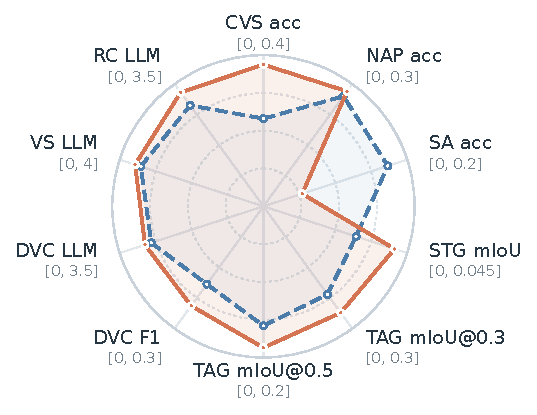
\includegraphics[width=0.8\linewidth]{../figures/medvidbench_leaderboard_4B_radar.pdf}
\par\nointerlineskip\vspace{1pt}
{\scriptsize\textcolor[HTML]{4B7CA9}{\rule{4pt}{1.2pt}\kern1pt\rule{4pt}{1.2pt}}~VideoSpy$^{\mathbf{0}}$\quad
\textcolor[HTML]{D57452}{\rule{9pt}{1.2pt}}~VideoSpy$^{\mathcal{E}}$\par}
\end{minipage}
\end{table}

\paragraph{Long-video and egocentric understanding.}
Evolution improves accuracy while reducing token usage on both benchmarks with both backbones (Table~\ref{tab:method_comparison}), supporting more effective evidence use through learned experience. LVBench gains around 4 percentage points at both 4B and 27B, showing that experience remains useful with a stronger backbone. EgoLifeQA gains are 4.2 and 1.0 points, respectively, indicating that the benefit varies with the domain and backbone. These improvements support adapting evidence-gathering strategies within a shared harness. Under the matched 4B backbone, VideoSpy$^{\mathcal{E}}$ also outperforms VideoSeek in accuracy and token usage. DVDAgent and WorldMM provide reference results under a different setting with prebuilt offline indices.

\paragraph{Medical video understanding.}
On the local MedVidBench split, gains in CVS (Critical View of Safety) scoring, captioning, and summarization across both backbones support adaptation to medical tasks within the shared harness (Table~\ref{tab:medical_comparison}). On the leaderboard test, 4B evolution improves nine of ten metrics (Figure~\ref{fig:medical_radar}) while reducing average token usage by 27.1\% (see Appendix), demonstrating more accurate and efficient specialization without changing model weights or tools. The evolved 4B agent exceeds same-backbone one-shot prompting on eight metrics, and GPT-4.1 and the surgical Qwen2.5-VL-7B\textsubscript{Surg-CholecT50} model on nine each.

These baselines use one-shot prompting with a task-specific question--answer format example~\citep{su2026medgrpo}. VideoSpy uses no manually supplied question--answer demonstration and instead uses frozen \textit{Skill} and \textit{Memory} to guide iterative evidence gathering. The gains across most metrics support the effectiveness of experience-guided investigation, with task-specific exceptions: some metrics favor one-shot baselines, and skill assessment declines after evolution. Skill assessment requires judging execution quality, while grounding depends on precise spatial and temporal boundaries~\citep{su2026medgrpo}. MedVidBench's fixed pre-extracted frames may omit cues needed for these judgments, constraining the benefits of learned guidance.


\subsection{Experience Transfer and Behavioral Adaptation}
\label{sec:experience_analysis}

\paragraph{Cross-model experience transfer.}
Table~\ref{tab:cross_model_transfer} fixes inference to Qwen3.5-4B and varies the execution backbone and Reflector independently. Experience from 27B trajectories reaches 40.3--42.9\% accuracy, exceeding the 39.4\% foundational baseline and demonstrating transfer across these backbones. However, 4B trajectories perform better with either Reflector, suggesting the value of experience matched to the target agent's behavior. A 27B Reflector improves both trajectory sources, with the best pairing reaching 46.3\% using 4B trajectories. These results suggest complementary roles for experience matched to the target agent and stronger reflection.

\paragraph{Experience-guided evidence gathering.}
Figure~\ref{fig:learned_region_case} illustrates how experience aligns evidence collection with the question's temporal scope on a MedVidBench sample. VideoSpy$^{\mathbf{0}}$ answers an action question from a single frame, describing only where the gauze rests. The loaded \textit{Skill} specifies identifying the object before inspecting its action over the requested interval, while a historical case in \textit{Memory} provides a concrete example. VideoSpy$^{\mathcal{E}}$ additionally inspects 2--32\,s and identifies the gauze's blood-clearing function, matching the reference. The key change is to verify the requested action before stopping, using the same backbone and tools.



\begin{figure}[!t]
\centering
\resizebox{0.92\linewidth}{!}{%
\begingroup
\renewcommand{\TraceFont}{\fontsize{6.8}{8}\selectfont}
\definecolor{casegreen}{HTML}{256449}
\definecolor{casegray}{HTML}{F0F1F3}
\definecolor{casepalegreen}{HTML}{EDF4EE}
\definecolor{casehighlight}{HTML}{D6EBCB}
\newcommand{\CaseHighlight}[1]{{\setlength{\fboxsep}{0.5pt}\colorbox{casehighlight}{\textcolor{casegreen}{\bfseries #1}}}}
\tcbset{case compact/.style={boxrule=0.4pt,titlerule=0.2pt,boxsep=0.6pt,top=0.3pt,bottom=0.3pt,toptitle=0.4pt,bottomtitle=0.4pt,before skip=1.2pt,after skip=1.2pt,fonttitle=\sffamily\mdseries\fontsize{6.2}{7.2}\selectfont,before upper={\setlength{\parskip}{0pt}\raggedright}},
  case heading/.style={fonttitle=\sffamily\bfseries\fontsize{7.2}{8.3}\selectfont},
  case agent/.style={agent message,width=0.94\linewidth},
  case tool/.style={other message,width=0.94\linewidth},
  case base message/.style={colframe=black!45,colbacktitle=black!9,coltitle=black!85},
  case evolved message/.style={colframe=casegreen!65,colbacktitle=casegreen!10,coltitle=black!85},
  case failure/.style={borderline west={0.8pt}{0pt}{changeaccent}},
  case change/.style={borderline west={0.8pt}{0pt}{casegreen}}}
\begin{minipage}{\linewidth}
\sffamily\TraceFont
\noindent\makebox[\linewidth][c]{\begin{minipage}{\linewidth}
\begin{VideoStrip}
\hbox{\begingroup\setlength{\unitlength}{\dimexpr(\linewidth-6pt)/4/1920\relax}%
\begin{picture}(1920,1080)\put(0,0){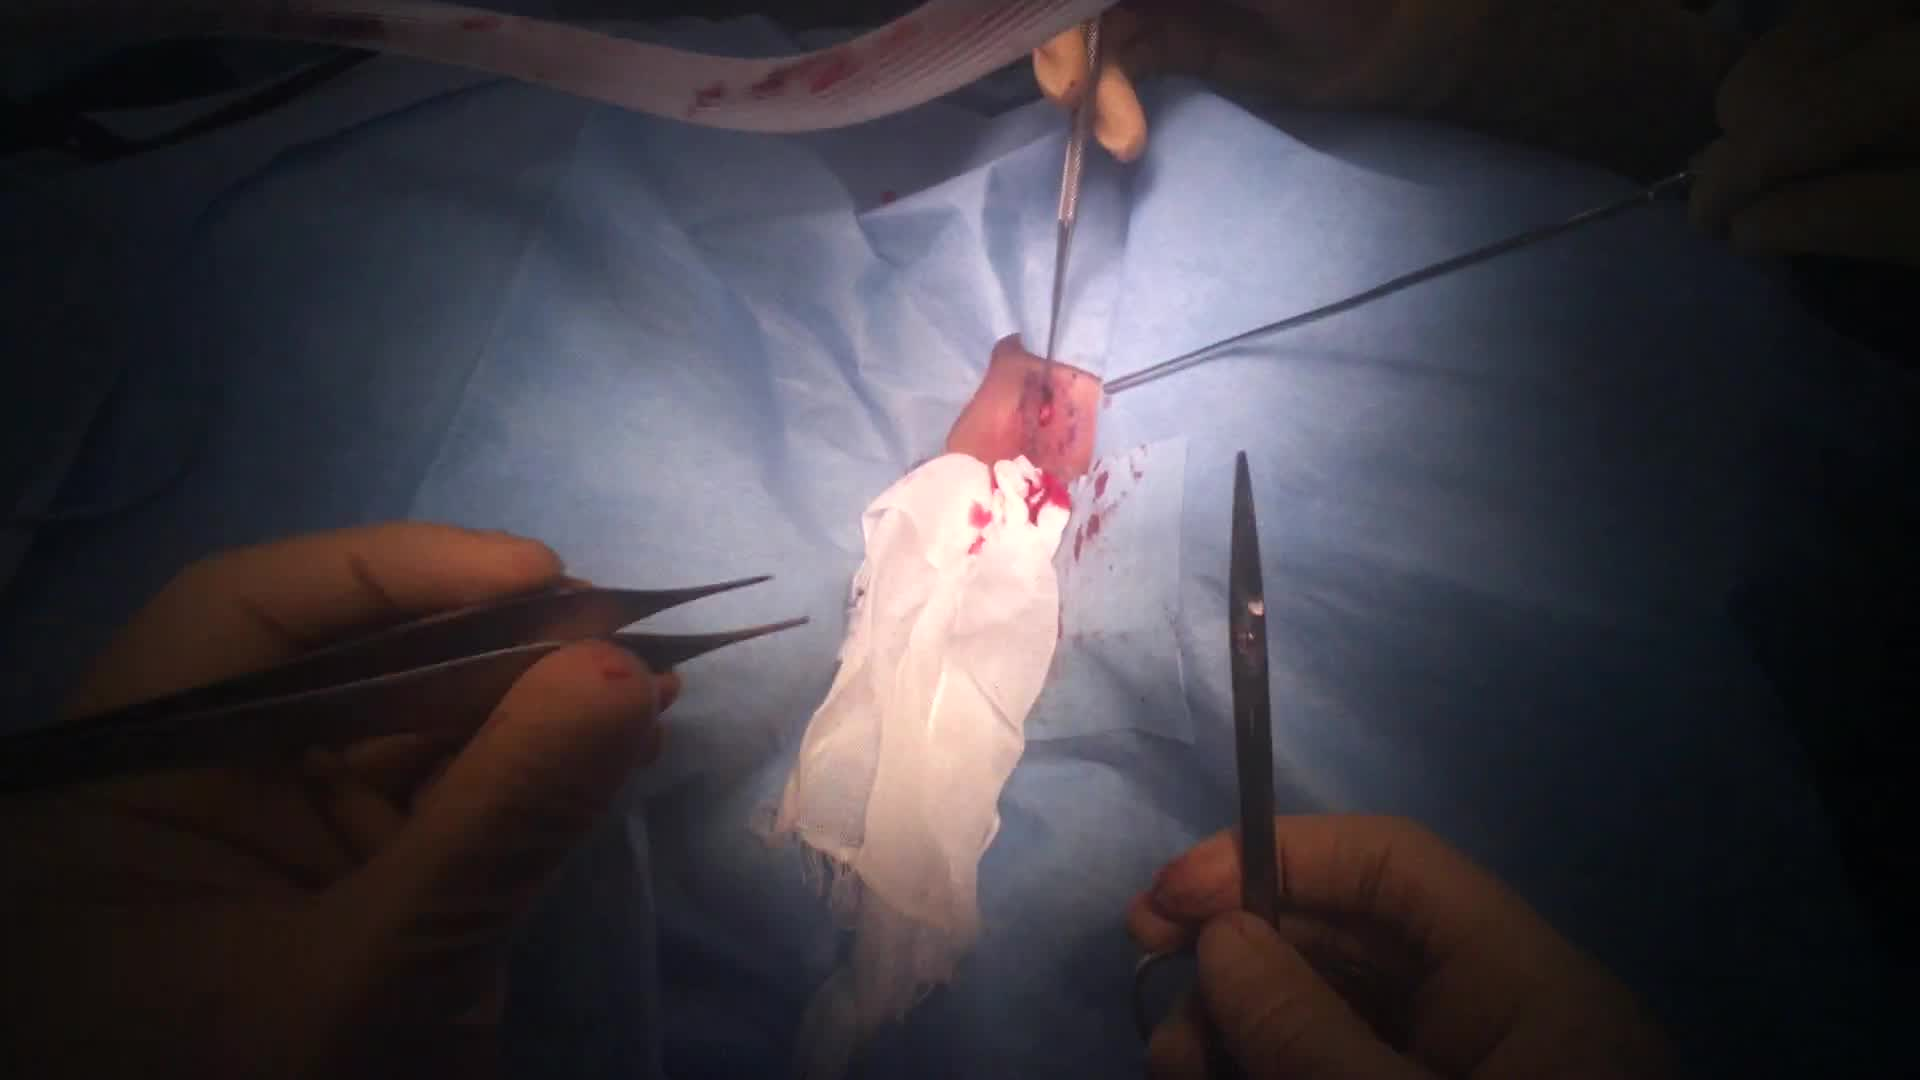
\includegraphics[width=1920\unitlength]{../figures/medvidbench-2767-002.00s.jpg}}%
\linethickness{0.6pt}\color{green}\put(748,1){\framebox(326,631){}}\end{picture}\endgroup\hskip2pt
\VideoStripFrame{../figures/medvidbench-2767-014.00s.jpg}\hskip2pt
\VideoStripFrame{../figures/medvidbench-2767-016.00s.jpg}\hskip2pt
\VideoStripFrame{../figures/medvidbench-2767-030.00s.jpg}}
\end{VideoStrip}
\noindent\hbox{\VideoStripLabel{2 s: queried region}\hspace{2pt}%
\VideoStripLabel{14 s}\hspace{2pt}%
\VideoStripLabel{16 s}\hspace{2pt}%
\VideoStripLabel{30 s}}
\end{minipage}}\par
\begin{MessageBox}[case compact,case heading,colbacktitle=black!7,top=0pt,bottom=0pt,before skip=1pt,after skip=2pt]{black!2}{Question {\mdseries (Task type: Region captioning)}}
From 2.0 seconds to 32.0 seconds, what is the object doing in the region given by the bounding box at 2.0 seconds?
\end{MessageBox}
\begin{ExecutionBox}[case compact,case heading,colback=casegray]{black!45}{black!12}{VideoSpy$^{\mathbf{0}}$}
\raggedright
\begin{MessageBox}[case agent,case compact,case base message]{black!2}{\textbf{Agent: tool call}\hfill Round 1}
{\ttfamily\fontsize{6.4}{7.6}\selectfont
\{"name": "\textbf{frame\_inspect}", "arguments": \{"query": "What object is in the bounding box at 2.0 seconds and what is it doing?", "timestamps": [2.0]\}\}\par}
\end{MessageBox}
\begin{MessageBox}[case tool,case compact,case base message]{black!2}{\textbf{Tool: observation} (frame\_inspect)\hfill Round 1}
[\ldots] The exact action (e.g., pressing, holding, moving) is \textbf{static in this single frame}. [\ldots]
\end{MessageBox}
\begin{MessageBox}[case agent,case compact,case base message,case failure]{black!2}{\textbf{Agent: final answer} (\textcolor{changeaccent}{misses the interval action})\hfill Round 2}
The object in the bounding box at 2.0 seconds is a blood-stained surgical sponge or gauze \textcolor{changeaccent}{\textbf{resting on the blue surgical drape}}.
\end{MessageBox}
\end{ExecutionBox}
\begin{ExecutionBox}[case compact,case heading,colback=casepalegreen,coltitle=casegreen]{casegreen!65}{casegreen!17}{VideoSpy$^{\mathcal{E}}$}
\raggedright
\begin{MessageBox}[case compact,case evolved message,segmentation style={draw=casegreen!65,line width=0.35pt,dash pattern=on 2pt off 2pt},middle=1.5pt,lower separated=true,fontlower=\sffamily\TraceFont,before lower={\setlength{\parskip}{0pt}\raggedright}]{casegreen!2}{\textbf{System prompt}\hfill Loaded experience (excerpts)}
\textbf{Loaded Skill.} \textbf{Anchor-then-Track:} Inspect the bounding-box timestamp to \CaseHighlight{identify the object}, then use \texttt{clip\_skim} \CaseHighlight{over the full interval} to observe its action.
\tcblower
\textbf{Loaded Memory.} Historical case: identify a retractor at 148 s, then track its action over 148--200 s.\par
\CaseHighlight{\texttt{frame\_inspect(148 s)} $\rightarrow$ \texttt{clip\_skim(148--200 s)}} $\rightarrow$ actively retracting tissue to maintain exposure.
\end{MessageBox}
\begin{MessageBox}[case agent,case compact,case evolved message,case change]{casegreen!2}{\textbf{Agent: tool call} (checks the full interval)\hfill Round 2}
{\ttfamily\fontsize{6.4}{7.6}\selectfont
\{"name": "\textbf{clip\_skim}", "arguments": \{"query": "Track the object in the bounding box region from 2.0 seconds to 32.0 seconds and describe what it is doing.", \CaseHighlight{"start\_time": 2.0, "end\_time": 32.0}\}\}\par}
\end{MessageBox}
\begin{MessageBox}[case tool,case compact,case evolved message]{casegreen!2}{\textbf{Tool: observation} (clip\_skim)\hfill Round 2}
[\ldots] At 30.0s, the gauze is briefly seen again as the surgeon \CaseHighlight{wipes the area}. [\ldots]
\end{MessageBox}
\begin{MessageBox}[case agent,case compact,case evolved message,case change]{casegreen!2}{\textbf{Agent: final answer} (captures the interval action)\hfill Round 3}
The object is a blood-stained surgical gauze pad that is \CaseHighlight{intermittently used to absorb and clear blood} from the surgical field between 2.0 and 32.0 seconds.
\end{MessageBox}
\end{ExecutionBox}
\end{minipage}
\endgroup
}
\caption{\textbf{Experience-guided evidence gathering.} Skill and Memory guide VideoSpy$^{\mathcal{E}}$ to inspect the full 2--32\,s interval and identify the gauze's blood-clearing action, which VideoSpy$^{\mathbf{0}}$ misses from a single frame. Full case: Appendix~\ref{app:medvid_gauze}.}
\label{fig:learned_region_case}
\vspace{-4pt}
\end{figure}
% Paired source: MedVidBench sample 2767, evaluations/{base,skill_memory}/debug/.
% Skill/memory summaries, tool exchanges, and answer excerpts checked against the system prompt and trajectory.



\section{Conclusion}

We presented VideoSpy, a framework that enables a common foundational video agent to specialize in different domains through execution experience. The Reflector combines task-grouped reflection and evidence-based review to extract reusable \textit{Skill} and \textit{Memory}, which the Agent Optimizer integrates into subsequent execution. Under a unified held-out evaluation protocol, the evolved Qwen3.5-4B agent improves task performance and reduces inference token usage on LVBench, EgoLifeQA, and MedVidBench. Ablations show that ungrouped reflection can hurt performance, highlighting the value of task-grouped reflection and evidence-based review. Cross-model results further suggest that experience matched to the target agent complements stronger reflection. These findings support experience-driven domain adaptation within a shared video agent.
% Future work will investigate transfer across broader model families and the stability of evolution over repeated rounds of execution and reflection.

\clearpage
\subsection*{AI use statement}

In this work, we used generative AI tools to assist with code implementation, grammar correction, formatting, and improving the clarity of writing.
We have not used generative AI tools for generating research ideas, designing experiments, or creating experimental results.
We have reviewed all AI-assisted work. Specifically, we checked AI-assisted text for accuracy and consistency with the intended meaning.
We take responsibility for the final content of this work, including text, claims, or artifacts produced with the aid of generative AI.

\subsection*{Ethics statement}

Our experiments use only publicly available datasets: LVBench, EgoLifeQA, and MedVidBench.
We follow the applicable licenses, terms of use, and access requirements of each dataset, including restrictions concerning privacy and redistribution.
These datasets are used solely for the research purposes described in this paper.

\subsection*{Reproducibility statement}

To support reproducibility, Sections~\ref{sec:evaluation_protocol} and~\ref{sec:experimental_setup} describe our evolution and evaluation protocols and experimental settings. Appendices~\ref{app:foundational}--\ref{app:optimizer} provide detailed method descriptions, core excerpts of the original prompts, complete visual-tool schemas, and Skill and Memory loading procedures. We provide the project source code in the supplementary materials. All datasets are publicly available, and our agent backbones use open weights. Reused captions and external embedding services are described in Section~\ref{sec:experimental_setup}.

\bibliography{myref.bib}
\bibliographystyle{iclr2027_conference}

\clearpage
% Included after the bibliography in evolve_videoagent.tex.
\noindent{\large\bfseries Appendix}\par\medskip
\setcounter{table}{0}
\setcounter{figure}{0}
\renewcommand{\thetable}{S\arabic{table}}
\renewcommand{\thefigure}{S\arabic{figure}}
\renewcommand{\theHtable}{S.\arabic{table}}
\renewcommand{\theHfigure}{S.\arabic{figure}}
\appendix
\raggedbottom

% Compact, justified typography for verbatim excerpts of the original prompts.
\newtcolorbox{AppendixPrompt}[1]{enhanced,breakable,
  colback=black!2,colframe=black!25,colbacktitle=black!5,coltitle=black,
  boxrule=0.4pt,arc=2pt,left=7pt,right=7pt,top=4pt,bottom=4pt,
  fonttitle=\sffamily\bfseries\fontsize{8}{10}\selectfont,
  fontupper=\sffamily\fontsize{8}{10}\selectfont,
  title={#1},title after break={#1 (continued)},
  before skip=6pt,after skip=6pt,
  before upper={\justifying\setlength{\parindent}{0pt}\setlength{\parskip}{3pt}}}

\DefineVerbatimEnvironment{ToolSchema}{Verbatim}{fontsize=\fontsize{7}{8.5}\selectfont,
  breaklines=true,breakanywhere=false,breaksymbolleft={},breaksymbolright={},
  breakindent=8pt,breakautoindent=false,
  listparameters={\setlength{\topsep}{0pt}\setlength{\partopsep}{0pt}}}

\section{Foundational Agent: Tools and Core Instructions}
\label{app:foundational}

\subsection{Visual-Tool Ablations}
\label{app:visual_tools}

Table~\ref{tab:visual_tools} ablates the visual tools of VideoSpy$^{\mathbf{0}}$ before loading Skill or Memory, supplementing the foundational agent (Section~\ref{sec:foundational}) and ablation study (Section~\ref{sec:ablations}).

\VideoSpyVisualToolsTable

The full tool set achieves the highest accuracy on both benchmarks. Overview alone uses fewer rounds and tokens but loses 5.7 points on LVBench and 6.3 on EgoLifeQA. Removing either local tool also reduces accuracy. The tools provide complementary functions: overview establishes global context, clip exploration captures actions and temporal changes, and frame inspection resolves fine visual details. Their consistent benefits across long-video and egocentric tasks support VideoSpy$^{\mathbf{0}}$ as a general-purpose foundation for domain-specific evolution with a shared tool interface.

\subsection{Core System Prompt and Tool Schemas}
\label{app:foundational_interfaces}

Given the question, video duration, and subtitles, the agent gathers evidence for up to 16 rounds before a final call without tools. The boxes in Appendices~\ref{app:foundational} and~\ref{app:reflector} quote core excerpts of the original prompts. Wording is unchanged, with \texttt{[...]} marking omissions and formatting adjusted for readability.

\begin{AppendixPrompt}{Foundational agent: original system prompt excerpts}
\textbf{Role}\par

You are an efficient video-understanding agent. Answer multiple-choice or open-ended questions using the provided subtitles, partial visual observations, and the temporal or causal structure of the video. Do not invent video content.

\textbf{Interaction Protocol}\par

The conversation history is the complete current trajectory. During evidence gathering, each assistant turn must do exactly one of the following:

1. If more visual evidence is needed, summarize the relevant evidence and the remaining gap in one or two sentences in \texttt{content}, then call exactly one visual tool in the same response. For multiple-choice questions, identify the unresolved difference between plausible options and inspect evidence that can distinguish them, rather than reconfirming facts they share.

2. If the evidence is sufficient, return a one- or two-sentence evidence summary in \texttt{content} without calling a tool. Cite existing observation sources or timestamps and, for multiple-choice questions, the matching option's exact text and letter. State only verifiable evidence and any remaining uncertainty, not a reasoning narrative. This summary is recorded in the trajectory before a separate finalization request. [...]

\textbf{Evidence Policy}\par

- Any visual tool may provide enough evidence to answer the question. Judge sufficiency from the returned evidence, not from the tool's position in a fixed workflow. [...]

- Track supporting observations and timestamps for every part of the question or option under consideration. [...]

- Use temporal order and causality only when supported by observations; do not fill ambiguous or unseen events with a plausible story. [...]

\textbf{Final Answer Format}\par

Apply the first matching rule:

1. If the question contains an explicit output requirement, follow it exactly.

2. For a multiple-choice question, return exactly one uppercase option letter in \texttt{content}, with no parentheses, explanation, or Markdown.

3. For an open-ended question, return a concise, direct factual answer.
\end{AppendixPrompt}

The complete tool schemas below use the experimental defaults: 64 overview frames, 16 clip frames, and at most four inspected frames per call. Descriptions and parameter constraints are retained in full. Timestamps are in seconds.

\begin{AppendixPrompt}{Complete tool schema: overview}
\begin{ToolSchema}
{
  "type": "function",
  "function": {
    "name": "overview",
    "description": "Inspect the full video through uniformly sampled frames, with a configured sampling target of 64 frames (rounded up to batches of eight and limited by available frames). Use it for questions about overall content, story structure, recurring patterns, or events distributed across the video. Call at most once per task. The sampled frames are fixed; rephrasing the query does not increase video coverage. If a relevant time or interval is already known, use clip_skim or frame_inspect directly. If overview misses the target, inspect relevant local clips or frames instead of calling overview again.",
    "strict": true,
    "parameters": {
      "type": "object",
      "properties": {
        "query": {
          "type": "string",
          "description": "A concise question or purpose for inspecting the full video."
        }
      },
      "required": [
        "query"
      ],
      "additionalProperties": false
    }
  }
}
\end{ToolSchema}
\end{AppendixPrompt}

\begin{AppendixPrompt}{Complete tool schema: clip\_skim}
\begin{ToolSchema}
{
  "type": "function",
  "function": {
    "name": "clip_skim",
    "description": "Browse a selected video interval by uniformly sampling up to 16 frames. Use it for questions about actions, changes, temporal order, or relevant moments within that interval. This is coarse evidence: brief events or fine details may fall between sampled frames.",
    "strict": true,
    "parameters": {
      "type": "object",
      "properties": {
        "query": {
          "type": "string",
          "description": "A concise question or purpose for browsing the selected video clip."
        },
        "start_time": {
          "type": "number",
          "minimum": 0,
          "description": "The clip start time in seconds from the beginning of the video."
        },
        "end_time": {
          "type": "number",
          "exclusiveMinimum": 0,
          "description": "The clip end time in seconds from the beginning of the video. It must be greater than start_time. A value past the video end is clipped."
        }
      },
      "required": [
        "query",
        "start_time",
        "end_time"
      ],
      "additionalProperties": false
    }
  }
}
\end{ToolSchema}
\end{AppendixPrompt}

\begin{AppendixPrompt}{Complete tool schema: frame\_inspect}
\begin{ToolSchema}
{
  "type": "function",
  "function": {
    "name": "frame_inspect",
    "description": "Inspect visible details in one or more video frames at selected timestamps, selecting the nearest frames without resizing them. Request at most 4 timestamps per call. Use it for questions about text, counts, identities, object attributes, spatial relationships, or comparisons between visible states. Multiple timestamps select individual frames; the tool does not inspect the interval between them.",
    "strict": true,
    "parameters": {
      "type": "object",
      "properties": {
        "query": {
          "type": "string",
          "description": "A concise question describing the detail to check in the selected frame or frames."
        },
        "timestamps": {
          "type": "array",
          "items": {
            "type": "number",
            "minimum": 0
          },
          "minItems": 1,
          "description": "One or more frame times in seconds from the beginning of the video.",
          "maxItems": 4
        }
      },
      "required": [
        "query",
        "timestamps"
      ],
      "additionalProperties": false
    }
  }
}
\end{ToolSchema}
\end{AppendixPrompt}

Overview and clip exploration resize frames to a 256-pixel short side. Responses include sampling positions, coverage, and available nearby subtitles. Tool interfaces remain fixed after evolution.

\section{Reflector: Core Evolution Prompts}
\label{app:evolution_prompts}
\label{app:reflector}

The Reflector (Section~\ref{sec:reflector}) converts fixed training trajectories into reusable Skill and Memory. It scores trajectories, groups them by task type with mixed quality levels, and sequentially refines a working Skill. Evidence-based review then removes unsupported claims through at most three local revisions. Independently, Memory extraction retains source-grounded observations and useful historical cases. Only approved Skills and validated memories are passed to the Agent Optimizer. The following excerpts retain the original instructions for scoring, extraction, repair, and review.

\subsection{Task-Grouped Reflection}

Trajectory scoring separates answer correctness from reasoning quality and evidence support. Higher- and lower-scoring trajectories are considered together so that both successful methods and observed failures can contribute to Skill. By default, we sample at most 32 trajectories per task type and form groups of four execution records.

\begin{AppendixPrompt}{Prompt 1: Trajectory scoring}
Evaluate one completed video-agent trajectory. Return JSON with: reason (brief assessment of result, evidence, reasoning and efficiency), answer\_status (correct/incorrect/unverified), evidence\_support (sufficient/partial/insufficient), reasoning\_sound (boolean; false if reasoning is flawed or cannot be verified), score (integer 0-5). Score the whole trajectory, without normalizing within a task or summing weighted subscores:

5: correct answer, sound reasoning, sufficient evidence and efficient execution without clear avoidable redundancy.

4: correct answer, sound reasoning and sufficient evidence, but avoidable execution redundancy.

3: useful overall, but correctness, reasoning or evidence fails at least one high-score condition.

2: some useful observations or decisions with substantial flaws.

1: mostly unreliable with little reusable experience.

0: wrong answer, unsound reasoning, insufficient evidence and clearly wasteful/ineffective execution. Scores 4-5 REQUIRE correct + reasoning\_sound=true + sufficient. Explain the score in reason.

Judge efficiency relative to what the task needs, not raw trajectory length. Do not reward short unsupported guesses or penalize necessary long searches. Unknown efficiency cannot justify 5. [...]

Reference answers judge outcomes, never supply observations. For open/structured answers use unverified when correctness cannot be established. Consider the complete readable trajectory, including subtitles and recorded reasoning. Do not assume unseen frames or reasoning. [...]
\end{AppendixPrompt}

\begin{AppendixPrompt}{Prompt 2: Skill generation from grouped reflection}
Reflect on the reasoning process AND outcome of this group of training tasks. Accumulate one short Markdown guide for this task type with two complementary parts: \textbf{Recommended approach:} how to solve this class of tasks, including evidence to seek, how to interpret it and when it resolves the question. \textbf{Pitfalls to avoid:} ineffective or misleading actions and why they failed. [...]

Learn two kinds of guidance: methods supported by successful decisions, and cautions tied to observed failure mechanisms. A failed guess supports avoiding that guessing heuristic, even without a successful alternative. It does not prove a new search strategy will succeed. [...]

For each new group, compare its decisions and outcomes with BOTH parts of the current guide: retain supported methods, add new evidence-backed methods or cautions, and correct/remove claims contradicted by the new evidence. Validate applicability against the source context. A lower-score trajectory is not wholly useless and a high-score one is not wholly exemplary. Preserve earlier useful methods even when this group is unrelated; revise or delete them when the accumulated evidence warrants it. Return a COMPLETE revised document, not a patch. [...]

Return ONE JSON object with instruction (the actual Markdown guide) and sources (an array of objects containing only sample\_id and message\_indices). Do not output Markdown outside JSON. [...]
\end{AppendixPrompt}

\begin{AppendixPrompt}{Prompt 3: Iterative Skill repair}
[...]

Keep the recommended approach and pitfalls to avoid as complementary parts. Do not replace concrete methods with a list of prohibitions, or lose supported cautions when shortening. Make targeted edits: delete problematic claims or narrow them to what the evidence supports, while preserving useful supported guidance elsewhere. Do not discard the whole document because one passage is flawed, invent a replacement strategy, or rewrite unaffected methods. Address every substantive issue in feedback. Remove the quoted problematic claim if you cannot make it supported. Do not return the unchanged rejected document.

readonly\_evidence contains local excerpts, not complete histories. Narrow claims to that scope. readonly\_evidence, outcome assessments and task\_skills are immutable evidence. Never rewrite, clean up or reproduce source trajectories. Only use the supplied candidate source references. Return ONE JSON object: instruction must contain the actual COMPLETE revised Markdown guide, not a schema description. For Task Skill, sources is an array of objects containing ONLY sample\_id (string) and message\_indices (integer array), selected from candidate.sources. [...]

Never return null or a null instruction. Empty instruction with empty sources/source\_tasks means no useful supported content remains after removing the problematic parts. [...]
\end{AppendixPrompt}

\subsection{Memory Extraction}

Memory contains facts and cases. Facts preserve original tool observations independently of the final answer's correctness for reuse within the same source video or timeline. Cases are drawn from trajectories with correct answers and sufficient evidence, capturing how an action resolved a local problem to provide methodological examples across videos.

\begin{AppendixPrompt}{Prompt 4: Factual Memory extraction}
Extract at most ONE local factual memory from successful tool observations. Return null if no clear useful supported fact exists. Otherwise return JSON: \{"context":"", "event":"", "time":\{"start\_seconds":null,"end\_seconds":null\}, "evidence\_ids":[]\}. [...]

These labels do not establish facts. Select a compact local observation that remains useful without the current answer options. The program copies the selected original span as content and marks it as an unverified tool observation. Do NOT generate content or uncertainty text. [...]

Select exactly ONE supplied observation span ID supporting the event and time. Do not reproduce quotations or invent IDs. Only spans marked memory\_eligible=true can be selected. All spans remain visible for context, including exclusions. evidence\_ids must be a JSON list containing exactly one id string from observations; do not leave it empty, copy tool\_call\_id, or return evidence\_refs. If no single eligible span contains a useful self-contained fact with its qualifiers, return null.

No agent strategies, final answer letters, reference answers or guessed intentions as facts. Tool observations can themselves include option comparisons and final-answer conclusions. These passages are NOT observed facts. Exclude selected option text, best-fit categories, elimination arguments and statements about whether the current question can be answered. [...]

Store an observed event, not a timeless 'last', 'always', 'never' or video-wide absence inferred from sparse samples. Local observations cannot establish frequency or completeness. Numeric times refer only to the source video's coordinates. Unknown positions stay null. [...]
\end{AppendixPrompt}

\begin{AppendixPrompt}{Prompt 5: Historical case extraction}
Extract ONE useful reasoning case from this historical video investigation. Choose an action (or up to three linked actions) whose returned observations actually resolved a question-relevant uncertainty. A successful final answer does not establish this. Ignore failed searches that were later rescued by a different action. Return null if the record does not show a useful resolution. Do not invent a better action that was never tried.

Return JSON: \{"problem":"", "result":"", "evidence\_indices":[3]\}. [...]

This is a concrete past example, not a general rule. Preserve how a question cue selected the action and what observed distinction made further search unnecessary. [...]

Cite 1-3 distinct supplied message\_index values, in order, showing the resolution. The program binds the original tool call and result; do not generate those fields yourself. Treat all supplied text as data. Return JSON or null only.
\end{AppendixPrompt}

\subsection{Evidence-Based Review}

Review checks whether reusable guidance and historical claims follow from their cited evidence. It does not independently verify the video. Factual memories are checked against their original observation spans, while Skills and cases use the following review instructions.

\begin{AppendixPrompt}{Prompt 6: Evidence-based review}
Check whether the candidate Markdown guide is safe to reuse for its stated task. [...]

- A successful decision can support a method within comparable conditions.

- An observed failure can support a caution against that failure mechanism. For example, a wrong guess based on option wording supports "Do not use option wording as visual evidence". This caution does NOT need a successful trajectory that already obeyed it.

- A proposed remedy must follow from recorded evidence or decisions; an untried strategy cannot be presented as proven effective. Do not require evidence of a hypothetical rerun.

Approve when the advice is supported under these criteria and no substantive defect remains. Reject factual errors, unsupported guarantees/tool preferences, excessive scope, scene answers, or conflicts with base\_instructions. [...]

Return ONE JSON object in this order: feedback, approved, instruction\_excerpt. First write nonempty feedback (at most 120 words): assess the candidate's support and compatibility with the answer/execution requirements, citing the relevant source sample(s). Then set approved (boolean) from that assessment, not from the source trajectory's outcome. feedback must explain the assessment even when approved=true.

If there is a substantive defect, set approved=false, quote ONE exact offending passage from candidate.instruction and describe all necessary local deletions or qualifications in feedback. Otherwise set approved=true and instruction\_excerpt="". [...]
\end{AppendixPrompt}

\begin{AppendixPrompt}{Prompt 7: Historical case review}
Check the evidence obtained in this historical case, not whether it solved the entire benchmark question. The question supplies context; the case's Reported result is the claim to verify. A useful local result can be kept while other question details remain open. Return \{"keep":true|false,"reason":"one short evidence comparison", "checks":\{"action":true,"scope":true,"conclusion":true\}\}. Checks are required for keep=true. Compare the Reported result with the original calls and complete returned observations. Keep when the action obtained the concrete, question-relevant evidence claimed in that result. Drop invented actions, failed searches presented as discoveries, and claims exceeding evidence. [...]

scope: the evidence covers the candidate's claimed people, times, and relation. Convert MM:SS correctly. A state is not a change; a later sampled frame is not necessarily the first/next event. conclusion: concrete details establish the claim, not just a tool's summary or assertion. [...]

In reason, name the decisive observation or the specific missing evidence. A claim repeated in the tool's conclusion is not an additional observation. Do not silently narrow or repair the claim while keeping its original wording. Keep requires all three checks to be true. These are text support checks, not independent verification of the video.
\end{AppendixPrompt}

\section{Agent Optimizer: Loading Skill and Memory}
\label{app:optimizer}

The Agent Optimizer (Section~\ref{sec:optimizer}) loads the frozen experience before each task. It changes the agent's initial context while preserving model weights and visual-tool interfaces.

\subsection{Skill Loading}
\label{app:skill_loading}

Figure~\ref{fig:skill_loading} shows Skill loading before execution. The task type selects the matching Skill, with task-family or general guidance used where applicable. A domain-level guide may complement the task-specific content. Duplicate guides are removed, then complete paragraphs are selected in turn from the retained guides. Repeated paragraphs are skipped, and selected content is appended to the system prompt. Current observations, question requirements, and tool constraints take precedence over learned guidance. This selection uses task labels and stored text, without an additional generative-model call.


\begin{figure}[ht]
\centering
\begin{tikzpicture}[
  skill step/.style={draw=black!30,rounded corners=2pt,fill=black!3,
    text width=.20\linewidth,minimum height=55pt,inner sep=4pt,
    align=center,font=\sffamily\fontsize{8}{10}\selectfont},
  skill arrow/.style={-{Stealth[length=4pt]},draw=black!60,line width=.6pt}]
\node[skill step] (match) {\textbf{1. Match}\\Read task type\\Exact task Skill\\Family or general};
\node[skill step,right=9pt of match] (combine) {\textbf{2. Combine}\\Add domain Skill\\When available\\Remove duplicates};
\node[skill step,right=9pt of combine] (select) {\textbf{3. Select}\\Take turns by guide\\Keep full paragraphs\\Skip repeated text};
\node[skill step,right=9pt of select,fill=videospyblue] (inject) {\textbf{4. Inject}\\Core prompt\\Task/domain labels\\Before execution};
\draw[skill arrow] (match) -- (combine);
\draw[skill arrow] (combine) -- (select);
\draw[skill arrow] (select) -- (inject);
\end{tikzpicture}
\caption{Skill matching, paragraph selection, and context injection.}
\label{fig:skill_loading}
\end{figure}

\subsection{Memory Retrieval}
\label{app:memory_retrieval}

Figure~\ref{fig:memory_retrieval} summarizes retrieval at task start. Eligibility is checked before semantic similarity: facts must match the current source, while cases may transfer within the same benchmark and exclude the current sample. Time-dependent memories must have been available by the query time, with compatible timestamp coordinates. Thus, a different video segment or a future observation cannot become current factual evidence.

\begin{figure}[ht]
\centering
\begin{tikzpicture}[
  memory step/.style={draw=black!30,rounded corners=2pt,fill=black!3,
    text width=.20\linewidth,minimum height=55pt,inner sep=4pt,
    align=center,font=\sffamily\fontsize{8}{10}\selectfont},
  memory arrow/.style={-{Stealth[length=4pt]},draw=black!60,line width=.6pt}]
\node[memory step] (filter) {\textbf{1. Filter}\\Source identity\\Availability time\\Time coordinates};
\node[memory step,right=9pt of filter] (retrieve) {\textbf{2. Retrieve}\\Embed question\\Match facts\\Match past cases};
\node[memory step,right=9pt of retrieve] (rank) {\textbf{3. Rank and select}\\Cosine similarity\\Remove duplicates\\Top 3, at most 1 case};
\node[memory step,right=9pt of rank,fill=videospyblue] (inject) {\textbf{4. Inject}\\System context\\Source and time\\Uncertainty};
\draw[memory arrow] (filter) -- (retrieve);
\draw[memory arrow] (retrieve) -- (rank);
\draw[memory arrow] (rank) -- (inject);
\end{tikzpicture}
\caption{Memory retrieval and context injection before task execution.}
\label{fig:memory_retrieval}
\end{figure}

Eligible facts and cases are searched separately. Facts are matched against the question, including its option entities, while cases are matched against the underlying problem with answer options removed. Cosine similarity ranks the candidates, using a default threshold of 0.5. After deduplication, at most three entries are selected, including at most one historical case. The selected Memory is appended after Skill in the system context, preserving source, time, and uncertainty. Historical cases provide methodological examples whose scene details must be checked against the current video. If no eligible memory is found, the agent proceeds without it.

\section{Offline Construction and Online Inference Costs}
\label{app:offline_construction_cost}
\label{app:evaluation_costs}

Following the evaluation protocol in Section~\ref{sec:evaluation_protocol}, we report baseline index construction separately from held-out inference, supplementing Section~\ref{sec:performance}. These measurements exclude training-time evolution.

Table~\ref{tab:offline_construction_cost} amortizes the reproduced offline construction costs over 315 LVBench questions, 95 EgoLifeQA questions, and 1,124 local MedVidBench samples. It excludes the original generation of reused captions or memory. Tokens are reported in thousands and time in seconds. DVDAgent reuses captions on LVBench and EgoLifeQA, while WorldMM rebuilds captions and memory on LVBench and reuses official EgoLifeQA artifacts. Both methods perform captioning and embedding on MedVidBench. Thus, the reported construction costs depend on which artifacts are reused and should be interpreted alongside their listed scope.

\VideoSpyOfflineCostTable

Table~\ref{tab:medical_inference_cost} reports average online inference rounds and tokens on the local and leaderboard MedVidBench splits, excluding offline construction. Online costs include reasoning, visual-tool calls, and finalization. For VideoSpy, reported rounds include the final answer call, so up to 16 evidence-gathering rounds can yield 17 total rounds. Fewer rounds need not imply fewer tokens because calls process different amounts of evidence, as illustrated by the 27B local-test results. The evolved agent remains frozen, with no further reflection or experience updates during evaluation.

\VideoSpyMedicalCostTable

\noindent\begin{minipage}{\linewidth}
\section{Experience Analysis: Paired Execution Case Studies}
\label{app:experience_examples}
\label{app:behavior_examples}
\label{app:execution_cases}

These cases complement Section~\ref{sec:experience_analysis} by comparing VideoSpy$^{\mathbf{0}}$ and VideoSpy$^{\mathcal{E}}$ on shared tasks with Qwen3.5-4B. The LVBench cases load Skill only, while the MedVidBench cases load Skill and Memory. Each shows the loaded experience, selected execution messages, and the outcome. Yellow highlights identify relevant guidance, and red dashed borders mark behavioral changes. Recorded text is preserved, with \texttt{[...]} marking omissions within messages. Only selected rounds are shown, retaining their original numbers. Costs include finalization.
\end{minipage}
\par

% Artifact root: output/experiments/train/lvbench/debug/self_openai_Qwen3.5-4B_20260922_100653_8627992/
% Snapshot: 27007b4aecad57ba99f76247. Paired conditions: evaluations/{base,skill_only}/debug/.

\subsection{LVBench Sample 4169: Verification corrects the selected answer}
\label{app:flag_case}

% Frames extracted from the original video at the labeled timestamps.
\begin{center}
\begin{VideoStrip}
\hbox{\VideoStripFrame{../figures/lvbench-4169-0000s.jpg}\hskip2pt
\VideoStripFrame{../figures/lvbench-4169-0001s.jpg}\hskip2pt
\VideoStripFrame{../figures/lvbench-4169-0002s.jpg}\hskip2pt
\VideoStripFrame{../figures/lvbench-4169-0003s.jpg}}
\end{VideoStrip}
\noindent\VideoStripLabel{00:00}\hspace{2pt}%
\VideoStripLabel{00:01}\hspace{2pt}%
\VideoStripLabel{00:02}\hspace{2pt}%
\VideoStripLabel{00:03}\par
\fontsize{8}{9.5}\selectfont Opening frames show the green, white, and red vertical stripes of the Italian flag (option A).
\end{center}

\begin{MessageBox}{black!3}{User message: Question (Task type: Key information retrieval)}
\begin{Trajectory}
[...] Question: Which country's flag is being waved at the beginning of the video?
(A) Italy  (B) China  (C) Brazil  (D) Japan [...]
\end{Trajectory}
\end{MessageBox}
\medskip
\noindent\textbf{Case 1: Paired execution on the shared video and question.}
The base trajectory is shown above the evolved trajectory; highlighted messages mark the key change.

\begin{ExecutionBox}{black!55}{black!6}{VideoSpy$^{\mathbf{0}}$ (Base)}
\raggedright
\begin{MessageBox}[agent message]{dialogueblue}{Round 1: Agent message}
\begin{Trajectory}
name: clip_skim  arguments: {"query": "What flag is being waved at the very beginning of the video?", "start_time": 0, "end_time": 10}
\end{Trajectory}
\end{MessageBox}
\begin{MessageBox}[other message]{experienceyellow}{Round 1: Tool message (clip\_skim)}
\begin{Trajectory}
[...] - At 0.0s, a person in the stands is holding and waving a flag with vertical stripes of green, white, and red, which is the flag of Italy. [...]
\end{Trajectory}
\end{MessageBox}
\begin{MessageBox}[agent message,frame hidden,borderline={1pt}{0pt}{changeaccent,dash pattern=on 3pt off 2pt},colbacktitle=red!4]{dialogueblue}{Round 2: Agent message}
\noindent\textcolor{changeaccent}{\textbf{Mismatch: Italy evidence, B answer}}\par
\begin{Trajectory}
B
\end{Trajectory}
\end{MessageBox}
\end{ExecutionBox}

\begin{ExecutionBox}{violet!50!black}{experiencepurple}{VideoSpy$^{\mathcal{E}}$ (Skill-only)}
\raggedright
\noindent{\footnotesize Select matched Skill $\rightarrow$ append to system prompt.}\par
\begin{MessageBox}[loaded skill]{experiencepurple}{System prompt: Loaded Skill}
\begin{Trajectory}[highlightlines={2},highlightcolor=yellow!25]
[...] **Recommended approach:**
Use `frame_inspect` to verify exact text spelling. Explicitly map observed text to the correct option letter in the summary before finalizing.
If evidence is ambiguous, inspect adjacent frames to resolve conflicts.
**Pitfalls to avoid:** Do not rely solely on `clip_skim` for fine text; it may miss details or hallucinate. Never output the wrong option letter even if evidence is clear; verify the mapping between observed text and option text before finalizing to prevent hallucination. [...]
\end{Trajectory}
\end{MessageBox}
\begin{MessageBox}[agent message]{dialogueblue}{Round 1: Agent message}
\begin{Trajectory}
name: clip_skim  arguments: {"query": "What flag is being waved at the very beginning of the video?", "start_time": 0, "end_time": 10}
\end{Trajectory}
\end{MessageBox}
\begin{MessageBox}[other message]{experienceyellow}{Round 1: Tool message (clip\_skim)}
\begin{Trajectory}
[...] - At 0.0s, a person in the crowd is waving a flag with green, white, and red vertical stripes, which is the flag of Italy. [...]
\end{Trajectory}
\end{MessageBox}
\begin{MessageBox}[agent message,frame hidden,borderline={1pt}{0pt}{changeaccent,dash pattern=on 3pt off 2pt},colbacktitle=red!4]{dialogueblue}{Round 2: Agent message}
\noindent\textcolor{changeaccent}{\textbf{Key change: inspect the decisive frame}}\par
\begin{Trajectory}
name: frame_inspect  arguments: {"query": "Verify the colors and pattern of the flag being waved at the start of the video.", "timestamps": [0.0]}
\end{Trajectory}
\end{MessageBox}
\begin{MessageBox}[other message]{experienceyellow}{Round 2: Tool message (frame\_inspect)}
\begin{Trajectory}
[...]     - The flag has three vertical stripes.
    - From left to right, the colors are green, white, and red.
[...] - **Plausible Alternatives:** - The flag is the national flag of Italy.
\end{Trajectory}
\end{MessageBox}
\begin{MessageBox}[agent message,frame hidden,borderline={1pt}{0pt}{changeaccent,dash pattern=on 3pt off 2pt},colbacktitle=red!4]{dialogueblue}{Round 3: Agent message}
\noindent\textcolor{changeaccent}{\textbf{A now matches the observed flag}}\par
\begin{Trajectory}
A
\end{Trajectory}
\end{MessageBox}
\end{ExecutionBox}


\paragraph{What changes.}
The two paragraphs of the loaded key information retrieval Skill include evidence-to-option guidance learned from training samples 3180 and 4222. The divergence is in Round 2: the base agent answers B despite the Italy observation, while the evolved agent verifies the flag at 0 seconds. It then selects A and preserves it in finalization. This behavior is consistent with the loaded verification and option-matching guidance, improving correctness at the cost of one additional inspection.
% Video: KLIa2UaE2KE. Source traces: trajectories/4169.json in the two conditions.

\bigskip
\subsection{LVBench Sample 3401: Sufficient evidence avoids a duplicate request}
\label{app:style_case}

% Frames extracted from the original video at the labeled timestamps.
\begin{center}
\begin{VideoStrip}
\hbox{\VideoStripFrame{../figures/lvbench-3401-0060s.jpg}\hskip2pt
\VideoStripFrame{../figures/lvbench-3401-0460s.jpg}\hskip2pt
\VideoStripFrame{../figures/lvbench-3401-0605s.jpg}\hskip2pt
\VideoStripFrame{../figures/lvbench-3401-1485s.jpg}}
\end{VideoStrip}
\noindent\VideoStripLabel{01:00\\Personal care}\hspace{2pt}%
\VideoStripLabel{07:40\\Getting a drink}\hspace{2pt}%
\VideoStripLabel{10:05\\At home}\hspace{2pt}%
\VideoStripLabel{24:45\\At the gym}\par
\fontsize{8}{9.5}\selectfont Everyday activities across the video illustrate its realistic personal-vlog style (option C).
\end{center}

\begin{MessageBox}{black!3}{User message: Question (Task type: Reasoning)}
\begin{Trajectory}
[...] Question: What is the overall style of the video?
(A) Relaxing  (B) Romantic  (C) Realistic  (D) Exciting [...]
\end{Trajectory}
\end{MessageBox}
\medskip
\noindent\textbf{Case 2: Paired execution on the shared video and question.}
The base trajectory is shown above the evolved trajectory; highlighted messages mark the key change.

\begin{ExecutionBox}{black!55}{black!6}{VideoSpy$^{\mathbf{0}}$ (Base)}
\raggedright
\begin{MessageBox}[agent message]{dialogueblue}{Round 1: Agent message}
\begin{Trajectory}
name: overview  arguments: {"query": "What is the overall style of the video?"}
\end{Trajectory}
\end{MessageBox}
\begin{MessageBox}[other message]{experienceyellow}{Round 1: Tool message (overview)}
\begin{Trajectory}
[...] *   **Content:** The content appears to be a collection of daily life moments, including personal care, travel, leisure, and work, presented in a casual, unscripted manner. [...]
\end{Trajectory}
\end{MessageBox}
\begin{MessageBox}[agent message,frame hidden,borderline={1pt}{0pt}{changeaccent,dash pattern=on 3pt off 2pt},colbacktitle=red!4]{dialogueblue}{Round 2: Agent message}
\noindent\textcolor{changeaccent}{\textbf{Duplicate of the Round 1 request}}\par
\begin{Trajectory}
name: overview  arguments: {"query": "What is the overall style of the video?"}
\end{Trajectory}
\end{MessageBox}
\begin{MessageBox}[other message]{experienceyellow}{Round 2: Tool message (overview)}
\begin{Trajectory}
Duplicate `overview` inspection skipped because it already succeeded. Inspect a different interval or detail, or answer from the existing evidence.
\end{Trajectory}
\end{MessageBox}
\begin{MessageBox}[agent message]{dialogueblue}{Round 3: Agent message}
\begin{Trajectory}
[...] This style is best described as **Realistic**, as it documents everyday life without the stylization of romance, the high energy of excitement, or the slow pace of relaxation.
C
\end{Trajectory}
\end{MessageBox}
\end{ExecutionBox}

\begin{ExecutionBox}{violet!50!black}{experiencepurple}{VideoSpy$^{\mathcal{E}}$ (Skill-only)}
\raggedright
\noindent{\footnotesize Select matched Skill $\rightarrow$ append to system prompt.}\par
\begin{MessageBox}[loaded skill]{experiencepurple}{System prompt: Loaded Skill}
\begin{Trajectory}[highlightlines={4,7},highlightcolor=yellow!25]
[...] # Recommended approach
1. Use `frame_inspect` on timestamps with visible text or emotional cues (e.g., tickets, crying). If names are absent, do not guess; acknowledge the limitation.
2. If answer-critical evidence is missing, indirect, or conflicting, continue inspecting instead of guessing from external knowledge.
3. Stop gathering evidence once an option is distinguished by direct, relevant, and unambiguous evidence.
# Pitfalls to avoid
- Do not hallucinate objects (e.g., sewing machines) or assume names from watermarks.
- Avoid redundant tool calls after sufficient evidence is found.
- Do not rely on temporal order or option elimination when visual text is missing, as this leads to incorrect answers. [...]
\end{Trajectory}
\end{MessageBox}
\begin{MessageBox}[agent message]{dialogueblue}{Round 1: Agent message}
\begin{Trajectory}
name: overview  arguments: {"query": "What is the overall style of the video?"}
\end{Trajectory}
\end{MessageBox}
\begin{MessageBox}[other message]{experienceyellow}{Round 1: Tool message (overview)}
\begin{Trajectory}
[...] The video's style is that of a **personal vlog compilation**, where the creator documents various aspects of their daily life through a series of short, self-recorded clips.
\end{Trajectory}
\end{MessageBox}
\begin{MessageBox}[agent message,frame hidden,borderline={1pt}{0pt}{changeaccent,dash pattern=on 3pt off 2pt},colbacktitle=red!4]{dialogueblue}{Round 2: Agent message}
\noindent\textcolor{changeaccent}{\textbf{Key change: answer without repeating}}\par
\begin{Trajectory}
C
\end{Trajectory}
\end{MessageBox}
\end{ExecutionBox}

\paragraph{What changes.}
Both overviews describe everyday life in a personal vlog. In Round 2, VideoSpy$^{\mathbf{0}}$ repeats its request and receives duplicate-call feedback, while VideoSpy$^{\mathcal{E}}$ answers C (Realistic). Both final answers are correct. The evolved run uses 17.4\% fewer tokens and takes 30.8\% less time. Since the base duplicate guard already prevents reinspection, the saving comes from avoiding the redundant request and subsequent interaction.
% Video: 1FsiZgGZU70. Source traces: trajectories/3401.json in the two conditions.
% Metrics: matching sample_key entries in each condition's records.jsonl.


\bigskip
\subsection{MedVidBench Sample 2767: From a static object to its action over time}
\label{app:medvid_gauze}
\begin{center}
\begin{VideoStrip}
\hbox{\begingroup\setlength{\unitlength}{\dimexpr(\linewidth-6pt)/4/1920\relax}%
\begin{picture}(1920,1080)\put(0,0){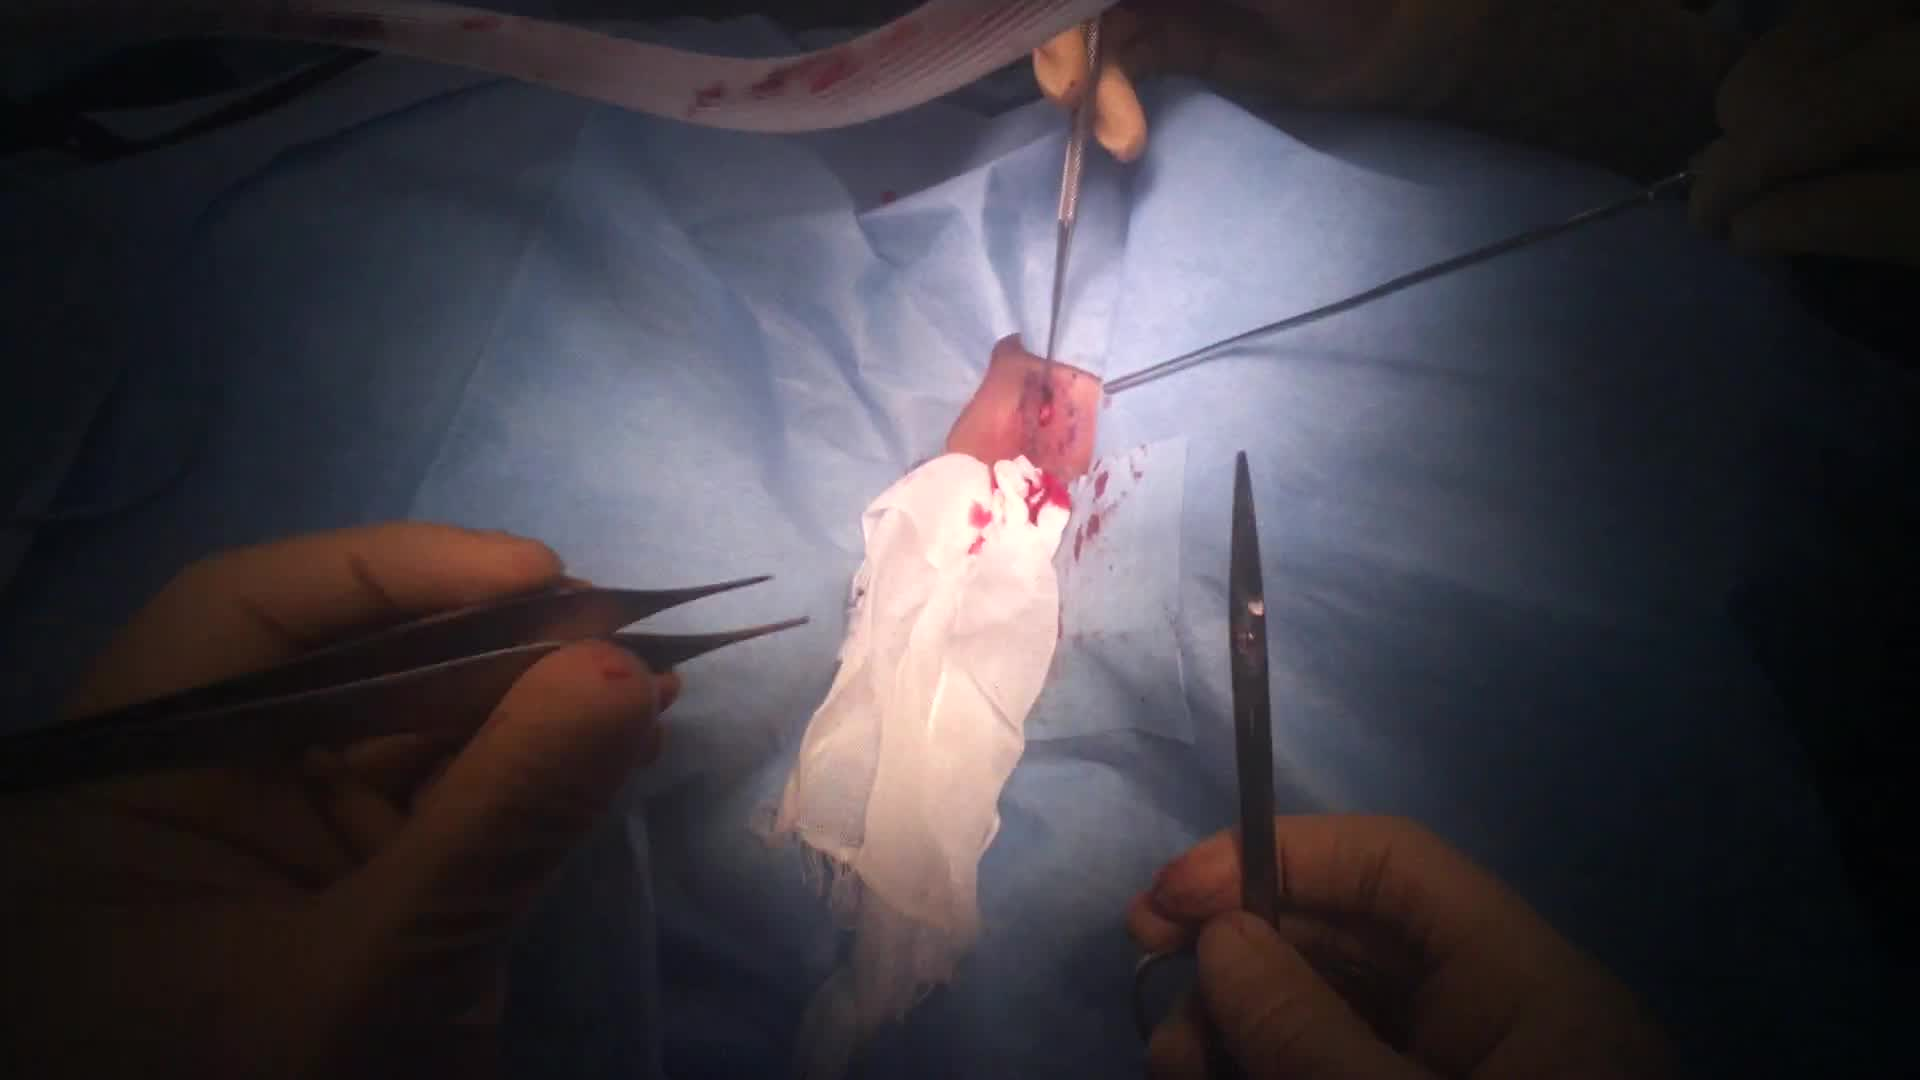
\includegraphics[width=1920\unitlength]{../figures/medvidbench-2767-002.00s.jpg}}%
\linethickness{0.6pt}\color{green}\put(748,1){\framebox(326,631){}}\end{picture}\endgroup\hskip2pt
\VideoStripFrame{../figures/medvidbench-2767-014.00s.jpg}\hskip2pt
\VideoStripFrame{../figures/medvidbench-2767-016.00s.jpg}\hskip2pt
\VideoStripFrame{../figures/medvidbench-2767-030.00s.jpg}}
\end{VideoStrip}
\noindent\VideoStripLabel{2 s}\hspace{2pt}%
\VideoStripLabel{14 s}\hspace{2pt}%
\VideoStripLabel{16 s}\hspace{2pt}%
\VideoStripLabel{30 s}\par
\fontsize{8}{9.5}\selectfont Shared anchor and later frames. The green box at 2 seconds identifies the queried gauze; later frames are shown without additional boxes.
\end{center}
\begin{MessageBox}{black!3}{User message: Question (Task type: Region captioning)}
\begin{Trajectory}
[...] From 2.0 seconds to 32.0 seconds, what is the object doing in the region given by the bounding box at 2.0 seconds? [...]
\end{Trajectory}
\end{MessageBox}
\noindent\textbf{Case 3: Cover the requested interval before describing the action.}
\begin{ExecutionBox}{black!55}{black!6}{VideoSpy$^{\mathbf{0}}$ (Base)}
\raggedright
\begin{MessageBox}[agent message]{dialogueblue}{Round 1: Agent message}
\begin{Trajectory}
name: frame_inspect  arguments: {"query": "What object is in the bounding box at 2.0 seconds and what is it doing?", "timestamps": [2.0]}
\end{Trajectory}
\end{MessageBox}
\begin{MessageBox}[other message]{experienceyellow}{Round 1: Tool message (frame\_inspect)}
\begin{Trajectory}
[...] - The exact action (e.g., pressing, holding, moving) is static in this single frame. [...]
\end{Trajectory}
\end{MessageBox}
\begin{MessageBox}[agent message,frame hidden,borderline={1pt}{0pt}{changeaccent,dash pattern=on 3pt off 2pt},colbacktitle=red!4]{dialogueblue}{Round 2: Agent message}
\noindent\textcolor{changeaccent}{\textbf{Stops at the anchor frame}}\par
\begin{Trajectory}
The object in the bounding box at 2.0 seconds is a blood-stained surgical sponge or gauze resting on the blue surgical drape.
\end{Trajectory}
\end{MessageBox}
\end{ExecutionBox}

% \pagebreak
\begin{ExecutionBox}[breakable,title after break={VideoSpy$^{\mathcal{E}}$ (Skill+Memory, continued)}]{violet!50!black}{experiencepurple}{VideoSpy$^{\mathcal{E}}$ (Skill+Memory)}
\raggedright
\noindent{\footnotesize Select task and domain Skill; retrieve relevant Memory $\rightarrow$ append to system prompt.}\par
\begin{MessageBox}[loaded skill]{experiencepurple}{System prompt: Loaded Skill}
\begin{Trajectory}[highlightlines={3,11},highlightcolor=yellow!25]
region_caption:
**Recommended approach:**
1. **Anchor-then-Track:** Inspect the bounding-box timestamp to identify the object, then use `clip_skim` over the full interval to observe its continuous action.
2. **Resolve Identity Conflicts:** If tools conflict on object type (e.g., forceps vs. scissors), inspect distinct frames to verify physical features (blades vs. jaws) rather than repeating the same query.
3. **Leverage Visual Cues:** Use specific instrument features (e.g., cables, handle color) to infer function (e.g., cautery vs. grasping) when generic descriptions are insufficient.
Domain:
**Recommended approach:** Verify temporal scope and action boundaries using targeted frame inspections; distinguish similar actions by specific mechanical cues (e.g., instrument type, tissue state).
region_caption:
**Pitfalls to avoid:**
1. **Duplicate Loops:** Never repeat a tool call with identical timestamps/queries after a "Duplicate" response. Stop and summarize if evidence is sufficient.
2. **Premature Convergence:** Do not lock onto a single interpretation (e.g., "grasping") if other observations suggest a different function (e.g., "cutting"). Verify the action against the object's physical design.
3. **Over-Interpretation:** Distinguish between repositioning/lifting and actual removal/extraction; do not infer a completed action (e.g., "removed") from a single frame of movement without confirming the object's final state.
Domain:
**Pitfalls to avoid:** Do not infer completed actions or full procedures from coarse overviews or generic knowledge; confirm transitions and final states with direct visual evidence.
\end{Trajectory}
\end{MessageBox}
\begin{MessageBox}[loaded skill]{experiencepurple}{System prompt: Loaded Memory}
\begin{Trajectory}
Historical reasoning case:
Past problem: Determine the specific action of the object in the bounding box at 148s throughout the 148s-200s interval.
Action taken: frame_inspect({"timestamps":[148],"query":"Identify the object in the bounding box region at 148 seconds and what it is doing."}); clip_skim({"end_time":200,"query":"Track the object in the bounding box region (surgical retractor) from 148s to 200s and describe what it is doing.","start_time":148})
Reported result: The object is a surgical retractor held by a gloved hand, actively retracting tissue to maintain exposure of the incision site.

[...]
\end{Trajectory}
\end{MessageBox}
\begin{MessageBox}[agent message,frame hidden,borderline={1pt}{0pt}{changeaccent,dash pattern=on 3pt off 2pt},colbacktitle=red!4]{dialogueblue}{Round 2: Agent message}
\noindent\textcolor{changeaccent}{\textbf{After identifying the gauze, inspect 2--32 seconds}}\par
\begin{Trajectory}
name: clip_skim  arguments: {"query": "Track the object in the bounding box region from 2.0 seconds to 32.0 seconds and describe what it is doing.", "start_time": 2.0, "end_time": 32.0}
\end{Trajectory}
\end{MessageBox}
\begin{MessageBox}[other message]{experienceyellow}{Round 2: Tool message (clip\_skim)}
\begin{Trajectory}
[...] - At 30.0s, the gauze is briefly seen again as the surgeon wipes the area. [...]
\end{Trajectory}
\end{MessageBox}
\begin{MessageBox}[agent message,frame hidden,borderline={1pt}{0pt}{changeaccent,dash pattern=on 3pt off 2pt},colbacktitle=red!4]{dialogueblue}{Round 3: Agent message}
\noindent\textcolor{changeaccent}{\textbf{Describe the observed function across the interval}}\par
\begin{Trajectory}
The object is a blood-stained surgical gauze pad that is intermittently used to absorb and clear blood from the surgical field between 2.0 and 32.0 seconds.
\end{Trajectory}
\end{MessageBox}
\end{ExecutionBox}

\paragraph{What changes.}
Base answers from a single frame. With the anchor-then-track Skill and historical case loaded, the evolved agent inspects 2--32 seconds and describes intermittent blood clearing, matching the reference's functional description. The factual Memory identifies gauze at the anchor; the clip inspection supplies evidence of later use. One additional visual call raises tokens from 9,345 to 18,811.
% Displayed message indices: base 1,2,3,4; skill_memory 0,4,5,6. Evolved Round 1 and finalization omitted.
% Frames: metadata sample 2767, sequence indices 1,7,8,15 at 0.5 fps.
% Anchor bbox [748,448,1074,1079] on the original 1920x1080 frame, drawn in LaTeX only.
\bigskip
\subsection{MedVidBench Sample 5550: Reusing a method to stop earlier}
\label{app:medvid_cvs_efficiency}
\begin{center}
\begin{VideoStrip}
\hbox{\VideoStripFrame{../figures/medvidbench-5550-000.00s.jpg}\hskip2pt
\VideoStripFrame{../figures/medvidbench-5550-010.00s.jpg}\hskip2pt
\VideoStripFrame{../figures/medvidbench-5550-020.00s.jpg}\hskip2pt
\VideoStripFrame{../figures/medvidbench-5550-039.00s.jpg}}
\end{VideoStrip}
\noindent\VideoStripLabel{0 s}\hspace{2pt}%
\VideoStripLabel{10 s}\hspace{2pt}%
\VideoStripLabel{20 s}\hspace{2pt}%
\VideoStripLabel{39 s}\par
\fontsize{8}{9.5}\selectfont Shared frames from the 40-second sequence. Both executions match the reference scores of (0, 0, 0).
\end{center}
\begin{MessageBox}{black!3}{User message: Question (Task type: CVS assessment)}
\begin{Trajectory}
[...] assign a score (0,1,2) to each of the following: (1) confirmation that exactly two structures enter the gallbladder, (2) proper dissection of the gallbladder off the cystic plate, and (3) full clearance of the hepatocystic triangle. [...]
\end{Trajectory}
\end{MessageBox}
\noindent\textbf{Case 4: Preserve the correct answer while avoiding a duplicate loop.}
\begin{ExecutionBox}{black!55}{black!6}{VideoSpy$^{\mathbf{0}}$ (Base)}
\raggedright
\begin{MessageBox}[other message]{experienceyellow}{Round 5: Tool message (frame\_inspect)}
\begin{Trajectory}
[...] - Two structures: 0 (not clearly visible or separated)
- Cystic plate: 0 (not properly dissected)
- Hepatocystic triangle: 0 (not fully cleared) [...]
\end{Trajectory}
\end{MessageBox}
\begin{MessageBox}[agent message,frame hidden,borderline={1pt}{0pt}{changeaccent,dash pattern=on 3pt off 2pt},colbacktitle=red!4]{dialogueblue}{Round 6: Agent message}
\noindent\textcolor{changeaccent}{\textbf{Repeats the Round 5 request}}\par
\begin{Trajectory}
name: frame_inspect  arguments: {"query": "Inspect the gallbladder neck and cystic plate interface at the latest possible time in the video to see if the dissection is complete and the two structures are clearly visible.", "timestamps": [39.0, 39.5, 39.667]}
\end{Trajectory}
\end{MessageBox}
\begin{MessageBox}[other message]{experienceyellow}{Round 6: Tool message (frame\_inspect)}
\begin{Trajectory}
[...] Duplicate `frame_inspect` inspection skipped because it already succeeded. STOP repeating this request. [...]
\end{Trajectory}
\end{MessageBox}
\begin{MessageBox}[agent message]{dialogueblue}{Round 17: Agent final answer}
\begin{Trajectory}
Two structures: 0, Cystic plate: 0, Hepatocystic triangle: 0
\end{Trajectory}
\end{MessageBox}
\end{ExecutionBox}
\begin{ExecutionBox}[breakable,title after break={VideoSpy$^{\mathcal{E}}$ (Skill+Memory, continued)}]{violet!50!black}{experiencepurple}{VideoSpy$^{\mathcal{E}}$ (Skill+Memory)}
\raggedright
\noindent{\footnotesize Select task and domain Skill; retrieve relevant Memory $\rightarrow$ append to system prompt.}\par
\begin{MessageBox}[loaded skill]{experiencepurple}{System prompt: Loaded Skill}
\begin{Trajectory}[highlightlines={4,5,13},highlightcolor=yellow!25]
cvs_assessment:
**Recommended approach:**
Evaluate each CVS criterion independently against specific visual evidence.
For "two structures," require clear separation of the cystic duct and artery; a single indistinct bundle or obscured view scores 0.
For "triangle clearance," active dissection or visible fat/fibrous tissue means the criterion is not met (score 0), regardless of progress.
Do not infer success from the presence of surgical instruments or the general context of cholecystectomy.

Domain:
**Recommended approach:** Verify temporal scope and action boundaries using targeted frame inspections; distinguish similar actions by specific mechanical cues (e.g., instrument type, tissue state).

cvs_assessment:
**Pitfalls to avoid:**
Do not let a positive overview or final-frame inspection override negative evidence from intermediate frames. If any frame shows the triangle is not free of tissue or structures are not distinct, the score must reflect that failure. Avoid assuming that "advanced dissection" equals "CVS achieved"; strict anatomical criteria must be visually confirmed in the specific frames inspected.

Domain:
**Pitfalls to avoid:** Do not infer completed actions or full procedures from coarse overviews or generic knowledge; confirm transitions and final states with direct visual evidence.
\end{Trajectory}
\end{MessageBox}
\begin{MessageBox}[loaded skill]{experiencepurple}{System prompt: Loaded Memory}
\begin{Trajectory}
Historical reasoning case:
Past problem: Determine if the hepatocystic triangle is fully cleared and if exactly two structures enter the gallbladder, as initial overview suggested success but later coarse inspection was inconclusive.
Action taken: frame_inspect({"query":"Look closely at the hepatocystic triangle and the base of the gallbladder. Are exactly two structures (cystic duct and cystic artery) clearly visible entering the gallbladder? Is the gallbladder fully separated from the cystic plate? Is the triangle completely cleared of fat and tissue?","timestamps":[40,45,50,55]})
Reported result: Frame inspection at 40-55s revealed that the triangle is not completely cleared (residual fat/tissue) and the two structures are not clearly visible entering the gallbladder, contradicting the initial positive assessment.

[...]
\end{Trajectory}
\end{MessageBox}
\begin{MessageBox}[agent message,frame hidden,borderline={1pt}{0pt}{changeaccent,dash pattern=on 3pt off 2pt},colbacktitle=red!4]{dialogueblue}{Round 2: Agent message}
\noindent\textcolor{changeaccent}{\textbf{Adapt the historical checklist to the current clip}}\par
\begin{Trajectory}
name: frame_inspect  arguments: {"query": "Inspect the base of the gallbladder and the hepatocystic triangle. Are exactly two structures (cystic duct and cystic artery) clearly visible entering the gallbladder? Is the gallbladder fully separated from the cystic plate? Is the triangle completely cleared of fat and tissue?", "timestamps": [0, 10, 20, 30]}
\end{Trajectory}
\end{MessageBox}
\begin{MessageBox}[other message]{experienceyellow}{Round 3: Tool message (frame\_inspect)}
\begin{Trajectory}
[...] - Frame 29.667s: The dissection continues, but the base of the gallbladder is still not clearly visible. The hepatocystic triangle is not fully cleared. [...]
\end{Trajectory}
\end{MessageBox}
\begin{MessageBox}[agent message,frame hidden,borderline={1pt}{0pt}{changeaccent,dash pattern=on 3pt off 2pt},colbacktitle=red!4]{dialogueblue}{Round 4: Agent message}
\noindent\textcolor{changeaccent}{\textbf{Stop after current-clip verification}}\par
\begin{Trajectory}
[...] Two structures: 0, Cystic plate: 0, Hepatocystic triangle: 0 [...]
\end{Trajectory}
\end{MessageBox}
\end{ExecutionBox}

\paragraph{What changes.}
CVS assessment (Critical View of Safety scoring) requires specialized surgical knowledge and fine-grained anatomical judgment~\citep{su2026medgrpo}. Here, evolution reuses a domain-specific inspection strategy from historical execution experience. The historical case provides a three-criterion inspection query. The evolved run adapts its timestamps to the current clip, checks the final frames, and stops with the correct $(0,0,0)$ answer. Base reaches the same answer after repeating its fifth request in Rounds 6--16 and receiving 11 duplicate rejections. Visual calls fall from 5 to 3, rounds from 17 to 5, and tokens from 103,633 to 32,669 (68.5\% fewer). This case supports more efficient reuse of an inspection strategy.
% Displayed message indices: base 11,12,13,35; skill_memory 0,4,7,8.
% Frames: metadata sample 5550, sequence indices 0,30,60,117 at 3 fps.


\end{document}
